%% Computers & Chemical Engineering (Elsevier) — CAS double-column manuscript.
%% Built on the Elsevier CAS template (cas-dc.cls, LPPL). DRAFT SKELETON:
%% bracketed [[...]] items are placeholders; results/case-study are marked TODO.
%% Do NOT insert unverified numbers — pull them from docs/techref/validation.rst.
\documentclass[a4paper,fleqn]{cas-dc}

\usepackage[authoryear,longnamesfirst]{natbib}
\usepackage{amsmath}

% Figures live in a local figs/ dir at submission; the technical-reference
% figures are reused directly here while drafting.
\graphicspath{{figs/}{../techref/figures/}}

\begin{document}
\let\WriteBookmarks\relax
\def\floatpagepagefraction{1}
\def\textpagefraction{.001}

\shorttitle{An open CAPE-OPEN gas-permeation membrane unit operation}
\shortauthors{Andreasen}

\title[mode=title]{An open, CAPE-OPEN gas-permeation membrane unit operation for process simulators}
%% Alternative title:
%% \title[mode=title]{A portable CAPE-OPEN unit operation for multicomponent
%%   gas-permeation membranes with real-gas and non-isothermal effects}

%% ---- Authors (placeholders) -------------------------------------------------
\author[1]{Anders Andreasen}
\cormark[1]
\ead{anra@ors-consulting.com}
\credit{Conceptualization, Methodology, Software, Validation, Writing}

\affiliation[1]{organization={ORS Consulting},
            addressline={Borgergade 66 st.\ th.},
            city={Esbjerg},
            postcode={DK-6700},
            country={Denmark}}

\cortext[1]{Corresponding author}

%% ---- Abstract ---------------------------------------------------------------
\begin{abstract}
Membrane gas separation is increasingly attractive for natural-gas
sweetening, hydrogen recovery, air separation and post-combustion carbon
capture, yet general-purpose process simulators still lack rigorous,
reusable membrane models. We present an open-source unit operation for
multicomponent gas permeation that complies with the CAPE-OPEN standard and
therefore runs unchanged in any compliant process modelling environment.
The physics core implements cross-flow, co-current and counter-current
solution--diffusion models, with an optional real-gas fugacity driving
force and an optional adiabatic (Joule--Thomson) non-isothermal energy
balance; all thermodynamic properties are delegated to the host flowsheet's
property package through the CAPE-OPEN Material Object, so the unit carries
no thermodynamics of its own. The implementation is validated against
independent analytical and numerical benchmarks from the literature
(Section~\ref{sec:validation}) and illustrated on a flowsheet-level
carbon dioxide / methane separation case study (Section~\ref{sec:casestudy}).
The software is released under the MIT licence [[repository URL / DOI]].
\end{abstract}

%% ---- Highlights -------------------------------------------------------------
\begin{highlights}
\item Open CAPE-OPEN membrane unit op runs in any compliant process simulator
\item Thermodynamics delegated to the host property package (Material Object)
\item Real-gas fugacity driving force and adiabatic non-isothermal layer
\item Validated against multiple independent literature benchmarks
\end{highlights}

%% ---- Keywords ---------------------------------------------------------------
\begin{keywords}
gas separation membranes \sep solution--diffusion \sep CAPE-OPEN \sep
process simulation \sep open-source software
\end{keywords}

\maketitle

%% ============================================================================
\section{Introduction}\label{sec:intro}
Membrane gas separation is a compact and energy efficient technology that has
gained a firm position alongside absorption, adsorption and cryogenic
distillation for a range of industrial separations. Established and emerging
applications include natural gas sweetening, hydrogen recovery and
purification, nitrogen production from air, biogas upgrading and
post-combustion carbon dioxide capture
\citep{Bernardo2009,BakerLokhandwala2008,Merkel2010}. The separation is
commonly described by the solution-diffusion mechanism, in which each component
dissolves in the membrane and diffuses across it under a difference in chemical
potential \citep{wijmans1995,baker2004}. The achievable combination of
permeability and selectivity is bounded by the permeability/selectivity
trade-off summarised by the Robeson upper bound \citep{Robeson2008}, which
continues to guide both material development and process design.

Reliable process models of gas permeation modules have been available for
decades. \citet{weller1950} derived an analytical solution for cross-flow
permeation, and \citet{shindo1985} provided one-dimensional formulations for
the cross-flow, co-current, counter-current, one-side-mixing and
perfect-mixing patterns that remain a common validation reference. Hollow-fibre
permeators were treated by \citet{pan1986}, and the governing equations are
presented in standard textbooks \citep{geankoplis}. More detailed descriptions
have since been reported, including multicomponent hollow-fibre models
\citep{coker1998} and the two-dimensional spiral-wound model of
\citet{diaspinto2020}. The range of module models and the physical effects that
they include or omit are surveyed in a recent review by \citet{daconceicao2023}.
Most of these models express the driving force as a partial-pressure difference
and assume ideal-gas behaviour. \citet{dejaco2020} instead defined permeance in
terms of fugacities and solved the module equations with a Peng-Robinson
equation of state, and reported that the ideal-gas assumption can overpredict
the stage cut by more than 10 percent for a high-pressure propane and propylene separation. Real-gas behaviour
and, for high-pressure or condensable mixtures, the temperature change caused by
permeation \citep{fontoura2022} are therefore relevant to accurate module
predictions.

Despite the maturity of the underlying models, membrane gas separation remains
poorly supported in general-purpose process simulators. \citet{alqaheem2024accuracy}
notes that process simulators contain many unit operations such as distillation
columns and reactors but lack a membrane unit for gas separation, in part
because there is no standard membrane design and the performance depends on the setup. The same limitation is
reported for commercial tools by \citet{ahmad2012}, who states that a membrane
separation model is not available in the standard version of Aspen HYSYS and
must be added through a Visual Basic subroutine, and by
\citet{aziaba2022}, who observes that membrane models are represented in process
simulation tools mainly through commercial systems and are commonly delivered as
black-box models that cannot be inspected or modified. As a consequence, much of
the published work relies on general mathematical software rather than on process
simulators \citep{alqaheem2024accuracy}, which complicates the study of a
membrane together with the compressors, heat exchangers and recycle streams that
surround it in a complete flowsheet.

Several routes have been used to introduce a membrane unit into a flowsheet, each
with practical drawbacks. One route adds a custom unit operation to a commercial
simulator, for example the two-dimensional cross-flow model coded in Visual Basic
for Aspen HYSYS by \citet{ahmad2012}, the extension unit developed for Honeywell
UniSim by \citet{bocciardo2013}, and the co-current hollow-fibre unit implemented
in C++ for Aspen HYSYS through the CAPE-OPEN interface by \citet{salano2025}.
These implementations are tied to a licensed simulator, and their source code is
generally not released. A second route reconstructs a membrane inside the
simulator from a component splitter combined with a spreadsheet and adjust
functions, which is laborious and specific to the flowsheet at hand
\citep{alqaheem2024accuracy,alqaheem2021}. A third route keeps the calculation in an external
numerical environment and connects it to the simulator, as in the COCO membrane
model of \citet{alqaheem2024coco}, where the balances are coded in Scilab and
linked through the Scilab plug-in. Rigorous open implementations also exist
outside the simulators, including the DWSIM membrane model of \citet{aziaba2022},
which is distributed as Visual Basic source that the user compiles into a
simulator-specific library, the open-source Python package MemPy of
\citet{dejaco2020}, which requires a Python, Pyomo and IPOPT toolchain together
with an external linear-solver library, and the standalone optimisation program
of \citet{bozorg2019}. The openly available options therefore depend on an
external numerical environment such as Scilab, MATLAB, Visual Basic or Python
with a nonlinear solver, or require the user to recompile the model, whereas the
ready-to-use options are proprietary.

The CAPE-OPEN standard provides a way to decouple a unit operation from a
specific simulator \citep{cocolan_uo}. A unit operation that complies with the
standard can be used in any compliant process modelling environment and can
obtain the thermodynamic and physical properties of its streams from the
property package selected in the flowsheet. Among the compliant environments,
COCO and its flowsheet environment COFE are available free of charge and are
used in both industrial and academic work, and any CAPE-OPEN compliant
thermodynamic server or unit operation can be added to them
\citep{andreasenvanbaten2025}. A free flowsheet environment together with a
standard interface provides a suitable basis for a membrane unit operation that
is portable across simulators and that reuses the host thermodynamics instead of
carrying its own.

To the best of our knowledge, an openly available, ready-to-use and thoroughly
validated gas-permeation membrane unit operation for a free CAPE-OPEN process
modelling environment has not been reported. The purpose of the present paper is
to present such a unit operation. The model is provided as a compiled CAPE-OPEN
unit that is registered directly in COCO/COFE, and in any other compliant
environment, without recompilation and without a separate numerical environment
or an external optimisation solver. All thermodynamic and physical properties,
including fugacities, enthalpies and phase behaviour, are obtained from the
flowsheet property package through the CAPE-OPEN Material Object, so that the
unit inherits the real-gas description already selected for the flowsheet. The
unit supports the cross-flow, co-current and counter-current flow patterns,
allows the driving force to be evaluated either from partial pressures or from
real-gas fugacities, and includes an optional adiabatic energy balance that
accounts for the temperature change of the permeate. The physics are implemented
in a simulator-independent core that is validated against experimental data and
against established literature and textbook models, and the complete source code
is released under an open licence. The remainder of the paper describes the model
formulation, the numerical solution, the software architecture, the validation
against independent references, and an illustrative flowsheet application.

%% ============================================================================
\section{Model formulation}\label{sec:model}
The unit models an isothermal, steady-state gas permeation module operating by
the solution-diffusion mechanism. This section states the local transport law,
the two forms of the driving force, the local permeate relationship, and the
module balances for the three flow patterns, followed by the optional adiabatic
energy balance. The physics core works internally in SI molar units. The main
symbols are defined where they first appear and follow the usual membrane
conventions \citep{baker2004}.

\subsection{Local flux and driving force}\label{sec:model-flux}
In the solution-diffusion picture a penetrant dissolves into the upstream face
of the dense active layer, diffuses down its chemical-potential gradient, and
desorbs at the downstream face \citep{wijmans1995}. For an ideal-gas mixture
with a partial-pressure driving force, the steady local molar flux of component
$i$ through an active layer of thickness $\ell$ is

\begin{equation}\label{eq:flux}
J_i = \frac{\mathcal{P}_i}{\ell}\,\bigl(p_\mathrm{r}\,x_i - p_\mathrm{p}\,y_i\bigr)
    = Q_i\,\bigl(p_\mathrm{r}\,x_i - p_\mathrm{p}\,y_i\bigr),
\end{equation}

where $\mathcal{P}_i$ is the permeability, $Q_i = \mathcal{P}_i/\ell$ is the
permeance, $p_\mathrm{r}$ and $p_\mathrm{p}$ are the retentate-side and
permeate-side pressures, and $x_i$ and $y_i$ are the local retentate and
permeate mole fractions. The unit uses the permeance $Q_i$ as the input property,
one value per component. The ideal selectivity of $i$ over $j$ is the permeance
ratio $\alpha_{ij} = Q_i/Q_j$. Permeance is entered in the units common in the
membrane literature (GPU) and converted internally to SI.

For a real gas the thermodynamically consistent driving force is the fugacity
difference rather than the partial-pressure difference,

\begin{equation}\label{eq:flux-fug}
J_i = Q_i\,\bigl(\varphi_i^{\mathrm{r}}\,p_\mathrm{r} x_i
                 - \varphi_i^{\mathrm{p}}\,p_\mathrm{p} y_i\bigr),
\end{equation}

where $\varphi_i^{\mathrm{r}}$ and $\varphi_i^{\mathrm{p}}$ are the fugacity
coefficients on the retentate and permeate sides, obtained from the equation of
state selected in the flowsheet and tending to unity as pressure tends to zero.
The unit defaults to the fugacity form and delegates the coefficients to the
property package. In the default setting the coefficients are evaluated once at
feed conditions and held constant along the module, which is a first-order
correction that is adequate because the fugacity coefficient varies only weakly
with the modest composition change along a module and the permeate-side
coefficient tends to unity at low permeate pressure. If the property package
cannot supply fugacity coefficients, the unit reverts to the partial-pressure
form of Eq.~\eqref{eq:flux}. One caveat applies to the input permeances:
literature values are typically regressed against a partial-pressure driving
force, so the fugacity form is strictly consistent only with permeances taken at
low pressure ($\varphi \approx 1$) or themselves referred to fugacity; a permeance
fitted at high pressure already absorbs part of the non-ideality, and applying
$\varphi$ to it would count that effect twice.

\subsection{Local permeate composition and module balances}\label{sec:model-balances}
The composition of the permeate crossing the membrane at a given position is the
flux fraction $J_i/\sum_k J_k$. In \emph{cross-flow} this freshly formed permeate
is swept away as it forms, so it also sets the local low-pressure partial pressure
in the driving force, and the permeate composition is the self-consistent flux
fraction $y_i = J_i/J_\mathrm{tot}$. Writing $S_i = Q_i/Q_1$ for the permeance
ratios and $\gamma = p_\mathrm{p}/p_\mathrm{r}$ for the pressure ratio, this gives
the cross-flow local permeate relationship

\begin{equation}\label{eq:yi}
y_i = \frac{S_i\,(x_i - \gamma\,y_i)}{\sum_k S_k\,(x_k - \gamma\,y_k)},
\end{equation}

in which the unknown appears on both sides through the downstream partial
pressure. Equation~\eqref{eq:yi} is the multicomponent generalisation of the
classical binary local permeate relationship \citep{weller1950}. It is written
here for the partial-pressure driving force; with the default fugacity driving
force of Eq.~\eqref{eq:flux-fug} the same relation holds because
$S_i(\varphi_i^{\mathrm{r}} x_i - \gamma\,\varphi_i^{\mathrm{p}} y_i) =
\tilde{S}_i(x_i - \tilde{\gamma}_i y_i)$, with the rescaled permeance ratio
$\tilde{S}_i = S_i\,\varphi_i^{\mathrm{r}}$ and the component-wise pressure ratio
$\tilde{\gamma}_i = \gamma\,\varphi_i^{\mathrm{p}}/\varphi_i^{\mathrm{r}}$ (the
partial-pressure case is $\varphi_i \equiv 1$). Equation~\eqref{eq:yi} is solved
at every position by the reformulated solver of Section~\ref{sec:numerics}. In the
co- and counter-current patterns (Section~\ref{sec:model-patterns}) the driving
force instead uses the bulk permeate composition, and $y_i$ in
Eq.~\eqref{eq:flux} denotes that bulk value.

Integrating the local flux over the module, with area $a$ measured from the feed
end and $R(a)$ the local retentate molar flow, gives the general retentate-side
balances

\begin{equation}\label{eq:mass-balance}
-\,\frac{\mathrm{d}R}{\mathrm{d}a} = J_\mathrm{tot}(a), \qquad
-\,\frac{\mathrm{d}(R\,x_i)}{\mathrm{d}a} = J_i(a),
\end{equation}

with $J_\mathrm{tot} = \sum_k J_k = \sum_k Q_k (p_\mathrm{r} x_k - p_\mathrm{p} y_k)$
and $J_i$ the component flux of Eq.~\eqref{eq:flux}. Only in cross-flow does the
second balance reduce to $-\,\mathrm{d}(R x_i)/\mathrm{d}a = y_i\,J_\mathrm{tot}$,
where $y_i = J_i/J_\mathrm{tot}$; in the other patterns the component flux $J_i$
is used directly. The overall stage cut, the single most important design
variable, is the fraction of the feed that permeates,
$\theta = \bigl(F - R(A)\bigr)/F$, with $F$ the feed molar flow and $A$ the total
membrane area.

\subsection{Flow patterns}\label{sec:model-patterns}
The way the permeate side is treated distinguishes the three flow patterns
\citep{shindo1985,pan1986}. In \emph{cross-flow}, the realistic idealisation for
spiral-wound modules \citep{baker2004,diaspinto2020}, the permeate formed at a point leaves
normal to the membrane and is swept away without mixing with permeate formed
elsewhere, so the local driving force uses only the local retentate composition.
For cross-flow the two balances in Eq.~\eqref{eq:mass-balance} combine, after
eliminating the total flux, into a single composition equation in which area
does not appear,

\begin{equation}\label{eq:cf}
\frac{\mathrm{d}x_i}{\mathrm{d}R} = \frac{y_i - x_i}{R}.
\end{equation}

The composition trajectory therefore depends only on the cut and not on the
absolute permeance level or the membrane area. The area required to reach a given
retentate flow is recovered by the quadrature
$A = \int_{R(A)}^{F} \mathrm{d}R / J_\mathrm{tot}\bigl(x(R)\bigr)$, and the
collected (product) permeate composition follows from an overall balance between
the feed and the local retentate,

\begin{equation}\label{eq:collected}
y_i^{\mathrm{coll}}(\xi) =
\frac{z_i - x_i(\xi)\,\bigl(1 - \theta(\xi)\bigr)}{\theta(\xi)},
\end{equation}

where $\xi = a/A$ is the dimensionless position, $z_i$ the feed composition and
$\theta(\xi)$ the cumulative cut. In the \emph{co-current} and
\emph{counter-current} patterns the permeate flows alongside the feed as a bulk
stream and the driving force uses the bulk permeate composition on the
low-pressure side. The permeate-side balances then read
$\mathrm{d}V/\mathrm{d}a = \pm J_\mathrm{tot}$ and
$\mathrm{d}(V y_i)/\mathrm{d}a = \pm J_i$, with the plus sign and the boundary
condition $V(0)=0$ for co-current, and the minus sign with $V(A)=0$ for
counter-current, $V(a)$ being the local permeate molar flow. For the same area,
feed and pressures the three patterns rank as
$\theta_\mathrm{counter} > \theta_\mathrm{cross} > \theta_\mathrm{co}$
\citep{shindo1985}. Cross-flow is the default and is a conservative
representation of spiral-wound duty, with counter-current available as the
best-case bound and co-current as the worst case. A schematic of the module and
its streams is shown in Fig.~\ref{fig:module}.

\begin{figure}[t]
  \centering
  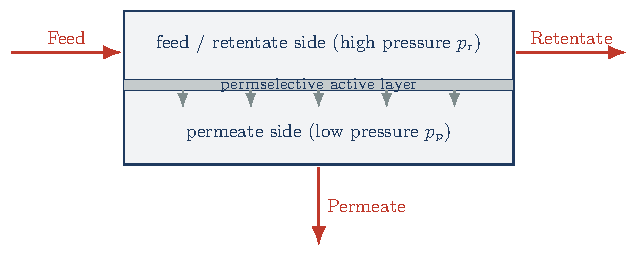
\includegraphics[width=0.8\linewidth]{tikz_module}
  \caption{Membrane module and stream definitions. The feed enters at high
  pressure $p_\mathrm{r}$; the retentate leaves at the same side, and the
  permeate is drawn across the active layer to the low-pressure side
  $p_\mathrm{p}$.}\label{fig:module}
\end{figure}

\subsection{Adiabatic energy balance}\label{sec:model-energy}
The separation is computed isothermally. The permeance is taken temperature
independent, and in the default fugacity mode the fugacity coefficients that enter
the driving force are evaluated once at the feed temperature
(Section~\ref{sec:model-flux}) and held fixed along the module, so the separation
does not respond to the temperature field; in the partial-pressure mode the
driving force carries no temperature dependence at all. An optional adiabatic energy balance is then
applied as a post-step that assigns outlet temperatures without changing the
separation. Crossing the membrane is treated as an isenthalpic (throttling) step:
the permeating gas retains the molar enthalpy it had on the high-pressure side
and is brought to the permeate pressure, which yields a Joule--Thomson
temperature change, while the retentate outlet temperature follows from the
overall adiabatic balance. With $h(T,p,\vec{x})$ the molar enthalpy from the
property package, $n_\mathrm{p} = F\theta$ and $n_\mathrm{r} = F(1-\theta)$,

\begin{equation}\label{eq:energy}
\begin{aligned}
h(T_\mathrm{p}, p_\mathrm{p}, \vec{y}) &= h(T_\mathrm{f}, p_\mathrm{r}, \vec{y}), \\
n_\mathrm{r}\,h(T_\mathrm{r}, p_\mathrm{r}, \vec{x}) &=
   F\,h(T_\mathrm{f}, p_\mathrm{r}, \vec{z}) - n_\mathrm{p}\,h(T_\mathrm{f}, p_\mathrm{r}, \vec{y}),
\end{aligned}
\end{equation}

which returns the permeate outlet temperature $T_\mathrm{p}$ and the retentate
outlet temperature $T_\mathrm{r}$. All enthalpies are taken from the property
package, so the Joule--Thomson behaviour is whatever the selected equation of
state implies; the unit does not hard-code a caloric correlation. Two points
follow from using a real equation of state. First, the reference enthalpy
$h(T_\mathrm{f}, p_\mathrm{r}, \vec{y})$ is that of the permeate-composition
mixture at the retentate pressure, a state the property package flashes and which,
for a condensable carbon-dioxide-rich permeate at high pressure, may lie in the
two-phase region. Second, the excess enthalpy of mixing then makes both outlet
temperatures differ from the feed temperature in general; the limit in which the
retentate returns exactly to the feed temperature (Section~\ref{sec:val-energy})
is specific to a fluid with no excess enthalpy of mixing, such as an ideal gas. A
fully resolved two-dimensional non-isothermal treatment of spiral-wound modules
is given by \citet{fontoura2022}; the present balance is a lumped adiabatic
reduction suited to a flowsheet unit. If the property package cannot deliver
enthalpies, the unit returns an isothermal result and records the reason.

\subsection{Assumptions}\label{sec:model-assumptions}
The model assumes steady state, constant per-component permeances (independent of
temperature, pressure and composition), and a negligible pressure drop along the
retentate channel. Any component whose local driving force would become negative
is capped at zero flux (no back-permeation). In cross-flow this cap never binds:
Eq.~\eqref{eq:yk-t} gives $x_i - \gamma y_i = x_i\,t/(t + S_i\gamma) \ge 0$, so the
local driving force is structurally non-negative. In the co- and counter-current
patterns, where the bulk permeate composition can locally exceed the retentate
partial pressure, the cap does bind and suppresses the physically real
back-permeation, a one-way-permeation approximation
(Section~\ref{sec:discussion}). The real-gas correction is applied to the driving
force only and not to the density and velocity balances or to a channel pressure
drop. The consequences of these assumptions are examined in
Sections~\ref{sec:validation} and~\ref{sec:discussion}.

%% ============================================================================
\section{Numerical solution}\label{sec:numerics}
The numerical schemes are chosen for robustness inside a flowsheet solver, where
a unit operation may be called many times with no opportunity for a user-supplied
initial guess. The schemes avoid initial guesses, avoid singularities at the
operating limits, and converge deterministically.

\subsection{Local permeate solver}\label{sec:numerics-local}
At every integration step the local permeate composition must be found from the
implicit set of Eq.~\eqref{eq:yi}. A direct fixed-point iteration becomes
ill-conditioned as the driving force vanishes (the pressure ratio approaching
unity, or near retentate exhaustion), where the common denominator collapses. The implementation instead reduces the problem to a single scalar
root-find. Introducing the scalar $t = \sum_k S_k (x_k - \gamma y_k)$, each
permeate mole fraction is explicit in $t$,

\begin{equation}\label{eq:yk-t}
y_k = \frac{S_k\,x_k}{t + S_k\,\gamma},
\end{equation}

and the closure $\sum_k y_k = 1$ becomes the single equation

\begin{equation}\label{eq:Ht}
H(t) = \sum_k \frac{S_k\,x_k}{t + S_k\,\gamma} - 1 = 0.
\end{equation}

For $0 < \gamma < 1$ (permeate pressure below the feed pressure and above
vacuum) and $t \ge 0$, every denominator $t + S_k\gamma$ is bounded below by
$S_k\gamma > 0$, so the singularity is removed. The function $H(t)$ is strictly
decreasing, is positive as $t \to 0^{+}$ and negative at $t = \sum_k S_k x_k$, so
the root is unique and bracketed in $\bigl(0, \sum_k S_k x_k\bigr)$; at the edges
$\gamma = 0$ or $\gamma = 1$ the root coincides with an endpoint of that interval. It is solved
by bisection with a Newton acceleration, the derivative
$H'(t) = -\sum_k S_k x_k / (t + S_k \gamma)^2$ being available in closed form,
which gives fast convergence with a guaranteed bracket. The permeate composition
then follows explicitly from Eq.~\eqref{eq:yk-t}. In the default fugacity mode the
same reduction is used with $S_k$ and $\gamma$ replaced by the rescaled
$\tilde{S}_k = S_k\varphi_k^{\mathrm{r}}$ and
$\tilde{\gamma}_k = \gamma\,\varphi_k^{\mathrm{p}}/\varphi_k^{\mathrm{r}}$ of
Section~\ref{sec:model-balances}, giving
$y_k = \tilde{S}_k x_k/(t + \tilde{S}_k\tilde{\gamma}_k)
= S_k\varphi_k^{\mathrm{r}} x_k/(t + S_k\gamma\varphi_k^{\mathrm{p}})$;
$H(t)$ remains strictly decreasing and bracketed in
$\bigl(0, \sum_k \tilde{S}_k x_k\bigr)$ when $0 < \tilde{\gamma}_k < 1$ for every
component.

\subsection{Integration of the module equations}\label{sec:numerics-march}
In design mode, where the target is a stage cut, the cross-flow composition
trajectory of Eq.~\eqref{eq:cf} is marched in the retentate flow $R$ from the
feed value downward with a fixed-step fourth-order Runge--Kutta scheme, the local
permeate solver being evaluated at each stage and the area accumulated by the
quadrature. In rating mode, where the membrane area is specified, the component
molar flows are integrated over area with an explicit first-order (forward Euler)
scheme at a fine step, marching until the accumulated area reaches the specified
value and interpolating the final partial step. Position profiles are recorded at
one hundred evenly spaced positions. The step counts are compile-time constants
set well beyond the point of diminishing returns. The quantitative benchmark
comparisons of Section~\ref{sec:validation} (Shindo, Weller--Steiner and the
air-separation experiment) are computed in design mode with the fourth-order
stage-cut march, which reaches an agreement of order $10^{-4}$. The first-order
rating march, used for area-specified solves and for the profiles, converges
first-order in the step count: for the Weller--Steiner case its outlet
composition approaches the fourth-order result with an error that halves as the
step count doubles, reaching about $1.5\times10^{-5}$ at the default of 4000 steps,
so it stays well below the benchmark tolerance and is not the accuracy
bottleneck.

The counter-current pattern is a two-point boundary-value problem, because the
permeate enters with zero flow at the retentate outlet while its composition at
the feed end is unknown. It is solved by an iterative cell march: the module is
discretised into cells, the permeate composition field is initialised from a
co-current or cross-flow pass, and the retentate and permeate profiles are swept
repeatedly in opposite directions until they stop changing to a set tolerance.
Co-current is a pure initial-value problem and needs a single forward sweep.

In design mode the required membrane area is found by an outer root-find. Because
the stage cut increases monotonically with area, an upper bound is grown
geometrically until the solved stage cut exceeds the target, after which the
bracket is bisected until the stage cut matches the target to a tolerance of
$10^{-6}$. Profiles are computed only once, for the final area, so the search
adds only a modest number of inexpensive solves.

\subsection{Temperature solve}\label{sec:numerics-temperature}
Each outlet temperature in Eq.~\eqref{eq:energy} is the solution of
$h(T,p,\vec{x}) = h_\mathrm{target}$. Molar enthalpy is monotone in temperature,
so the solve is a bracketed bisection with a secant hint, expanding an initial
bracket until it straddles the root and then contracting until the enthalpy
residual falls below $10^{-6}$ of its scale. The scheme uses only enthalpy
evaluations and does not require the property package to expose a
pressure-enthalpy flash, which is what makes the energy balance portable across
property packages. Profile temperatures reuse the previous point as a warm start
and converge in a few iterations.

%% ============================================================================
\section{Software architecture and implementation}\label{sec:software}
The software is organised as two assemblies with a strict dependency direction
(Fig.~\ref{fig:arch}). The core, \texttt{MembraneCore}, contains only the
numerical models of Sections~\ref{sec:model} and~\ref{sec:numerics}. It has no
COM, no CAPE-OPEN and no thermodynamics of its own; where it needs a fluid
property, namely enthalpy for the energy balance, it declares a narrow port
interface that the caller supplies. This allows the entire physics to be tested
in isolation on modern .NET. The adapter, \texttt{Membrane.CapeOpen}, is a .NET
Framework, x64, COM-visible assembly that implements the CAPE-OPEN interfaces,
translates the Material Objects presented by the environment to and from the
core's array-based interface, and delegates all thermodynamics to the property
package. The adapter depends on the core, and the core never depends on the
adapter, so the model can be moved to a non-CAPE-OPEN host by writing a new
adapter alone. This ports-and-adapters arrangement is the same one used in
related open thermodynamic components.

\begin{figure}[t]
  \centering
  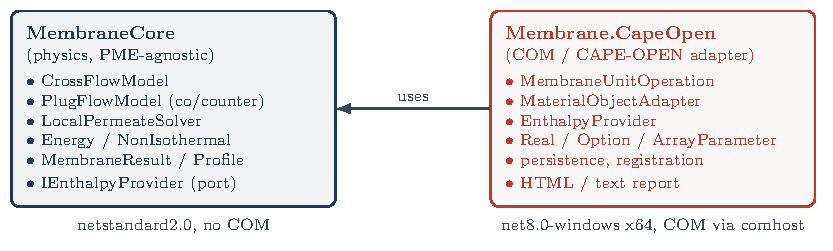
\includegraphics[width=\linewidth]{tikz_arch}
  \caption{The two-assembly architecture. The CAPE-OPEN adapter depends on the
  physics core; the core has no dependency on the adapter or on any
  simulator.}\label{fig:arch}
\end{figure}

\subsection{CAPE-OPEN interfaces and the solve lifecycle}\label{sec:software-co}
The unit is a CAPE-OPEN unit operation \citep{cocolan_uo}. The primary class
implements the interfaces listed in Table~\ref{tbl:interfaces}. Three material
ports are exposed, a feed inlet and retentate and permeate outlets. The
environment drives the standard lifecycle: a Material Object is connected to each
port, the unit is validated, and the unit is calculated. Validation checks that
the ports are connected, discovers the feed compound list, ensures that a
permeance parameter exists for every compound, and checks the operating
parameters. Validation reads only the compound list and never the stream state,
because temperature, pressure and composition are undefined until the flowsheet
is solved. On calculation the unit reads the feed state, solves the selected
model, and writes and flashes the two product streams.

\begin{table}[t]
\caption{CAPE-OPEN interfaces implemented by the unit
operation.}\label{tbl:interfaces}
\begin{tabular*}{\tblwidth}{@{}LL@{}}
\toprule
Interface & Role \\
\midrule
\texttt{ICapeUnit} & Ports, validation, calculation and status. \\
\texttt{ICapeIdentification} & Name and description shown in the palette. \\
\texttt{ICapeUtilities} & Initialisation, parameter collection, edit dialog and context. \\
\texttt{ICapeUnitReport} & Text and HTML result reports. \\
\texttt{IPersistStreamInit} & Save and load of the unit state in the flowsheet file. \\
\texttt{ECapeRoot}, \texttt{ECapeUser} & Readable error name and description. \\
\bottomrule
\end{tabular*}
\end{table}

Because the component set is unknown until a feed is connected, the permeance
parameters are created dynamically. On the first validation the adapter reads the
feed compound list and adds one permeance parameter per compound to the parameter
collection, seeding it from any persisted value. A specification-mode parameter
selects whether the membrane area or the stage cut is the specified quantity, and
switches the two parameters between input and output so that the environment
greys out the computed one. In design mode the calculation root-finds the area
that reaches the target stage cut and writes it back.

\subsection{Thermodynamic delegation}\label{sec:software-thermo}
All thermodynamics is delegated to the property package through the Material
Object. The adapter prefers the CAPE-OPEN 1.1 material interface and falls back
to the 1.0 interface when only that is offered. At calculation it reads the feed
temperature, pressure, composition and total flow from the feed object; it writes
each product by setting the overall state and then requesting a
temperature-pressure flash. The flash is treated as non-fatal: if the property
package declines it, the overall state has already been set and the environment
flashes the stream during the flowsheet solve. Fugacity coefficients for the
driving force of Eq.~\eqref{eq:flux-fug} and enthalpies for the energy balance of
Eq.~\eqref{eq:energy} are obtained through a private scratch Material Object
cloned from the feed, so the real streams are never disturbed. Before writing any
stream the unit probes once whether the property package can deliver the required
property, and falls back to the partial-pressure or isothermal path if it cannot,
recording the reason in a diagnostic log.

\subsection{Persistence, profiles and registration}\label{sec:software-persist}
Some environments perform the flowsheet solve in a separate worker instance of
the unit, distinct from the instance shown in the interface, so output values set
during calculation are not visible in the displayed instance unless they are
persisted and reloaded. The unit therefore serialises its full state, comprising
the operating parameters, the per-compound permeances, the computed stage cut and
the position profiles, through a save and load mechanism with an integer version
header, so that older flowsheet files load into newer builds. The unit reports
itself as always requiring persistence, because parameter values edited in the
environment grid update the parameter objects directly without notifying the
unit. Position profiles are exposed as array output parameters sampled at one
hundred points, so that the environment can plot concentration, stage-cut and
temperature profiles along the module; getting the array parameter contract right
\citep{cocolan_param,cocolan_param_errata} is what makes the profiles plot rather
than appear as invalid values. The unit registers per user, without administrator
rights, and an assembly resolver ensures the core library is found when the unit
is activated inside the environment process. Figure~\ref{fig:cofe} shows the unit
operating in COFE.

\begin{figure}[t]
  \centering
  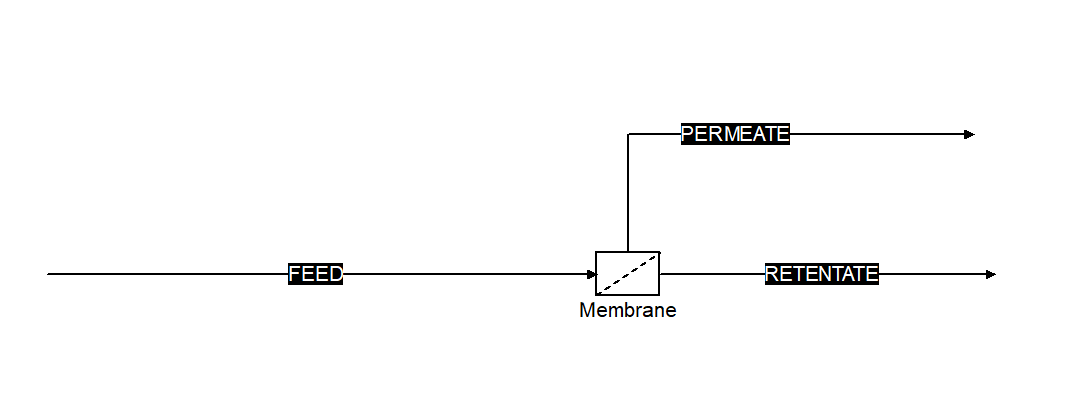
\includegraphics[width=\linewidth]{COFE_membrane}
  \caption{The membrane unit operation in the free COFE flowsheet environment,
  with feed, retentate and permeate streams and the parameter
  grid.}\label{fig:cofe}
\end{figure}

%% ============================================================================
\section{Validation}\label{sec:validation}
The unit is validated at several levels: an automated test suite over the physics
core and the adapter, reproduction of independent analytical and numerical
benchmarks, the analytic limits of the energy balance, and comparison with
experimental data. All figures in this section are produced by scripts that read
results written by the solver, so none of the reported numbers are entered by
hand. A suite of 54 automated tests runs on every build, 44 exercising the
physics core, including the local permeate solver over binary and multicomponent
feeds and the limiting pressure ratios, the flow-pattern ranking, the
collected-permeate balance and the energy-balance limits, and 10 exercising the
adapter, including the validation and calculation lifecycle, the
specification-mode round-trip and the save and load of the unit state.

\subsection{Multicomponent benchmark: Shindo et al.}\label{sec:val-shindo}
The multicomponent calculation methods of \citet{shindo1985} are the standard
one-dimensional benchmark, tabulated again by \citet{diaspinto2020}. Two cases
are reproduced. Case~1 is a ternary ammonia, hydrogen and nitrogen separation
through polyethylene at a pressure ratio of $0.13$; Case~2 is a five-component
hydrogen, methane, carbon monoxide, nitrogen and carbon dioxide separation
through microporous glass at a pressure ratio of $0.10$. The permeate
composition at the benchmark stage cut is reproduced to an absolute agreement of
order $10^{-4}$ for both cross-flow and counter-current, as shown in
Table~\ref{tbl:shindo} for Case~1 and in Fig.~\ref{fig:shindo}. Reproducing
Case~2 requires the hydrogen permeance to be taken as
$4.80\times10^{-10}$ rather than the
$4.80\times10^{-9}$~$\mathrm{mol\,m^{-2}\,s^{-1}\,Pa^{-1}}$ listed in the
tabulation of \citet{diaspinto2020}; with the larger value the reported
enrichment is unreachable, so it appears to be a factor-of-ten transcription
error in that reproduction of the Shindo case. The corrected value reproduces the
benchmark and preserves the expected ordering of the microporous-glass
permeances.

\begin{table}[t]
\caption{Shindo Case~1 permeate composition
(NH\textsubscript{3}/H\textsubscript{2}/N\textsubscript{2}) at the benchmark
stage cut.}\label{tbl:shindo}
\begin{tabular*}{\tblwidth}{@{}LLLL@{}}
\toprule
Pattern & Species & \citet{shindo1985} & This work \\
\midrule
Cross-flow            & NH\textsubscript{3} & 0.7338 & 0.7336 \\
($\theta=0.373$)      & H\textsubscript{2}  & 0.2035 & 0.2037 \\
                      & N\textsubscript{2}  & 0.0627 & 0.0627 \\
\addlinespace
Counter-current       & NH\textsubscript{3} & 0.7368 & 0.7367 \\
($\theta=0.375$)      & H\textsubscript{2}  & 0.2010 & 0.2011 \\
                      & N\textsubscript{2}  & 0.0622 & 0.0622 \\
\bottomrule
\end{tabular*}
\end{table}

\begin{figure*}[t]
  \centering
  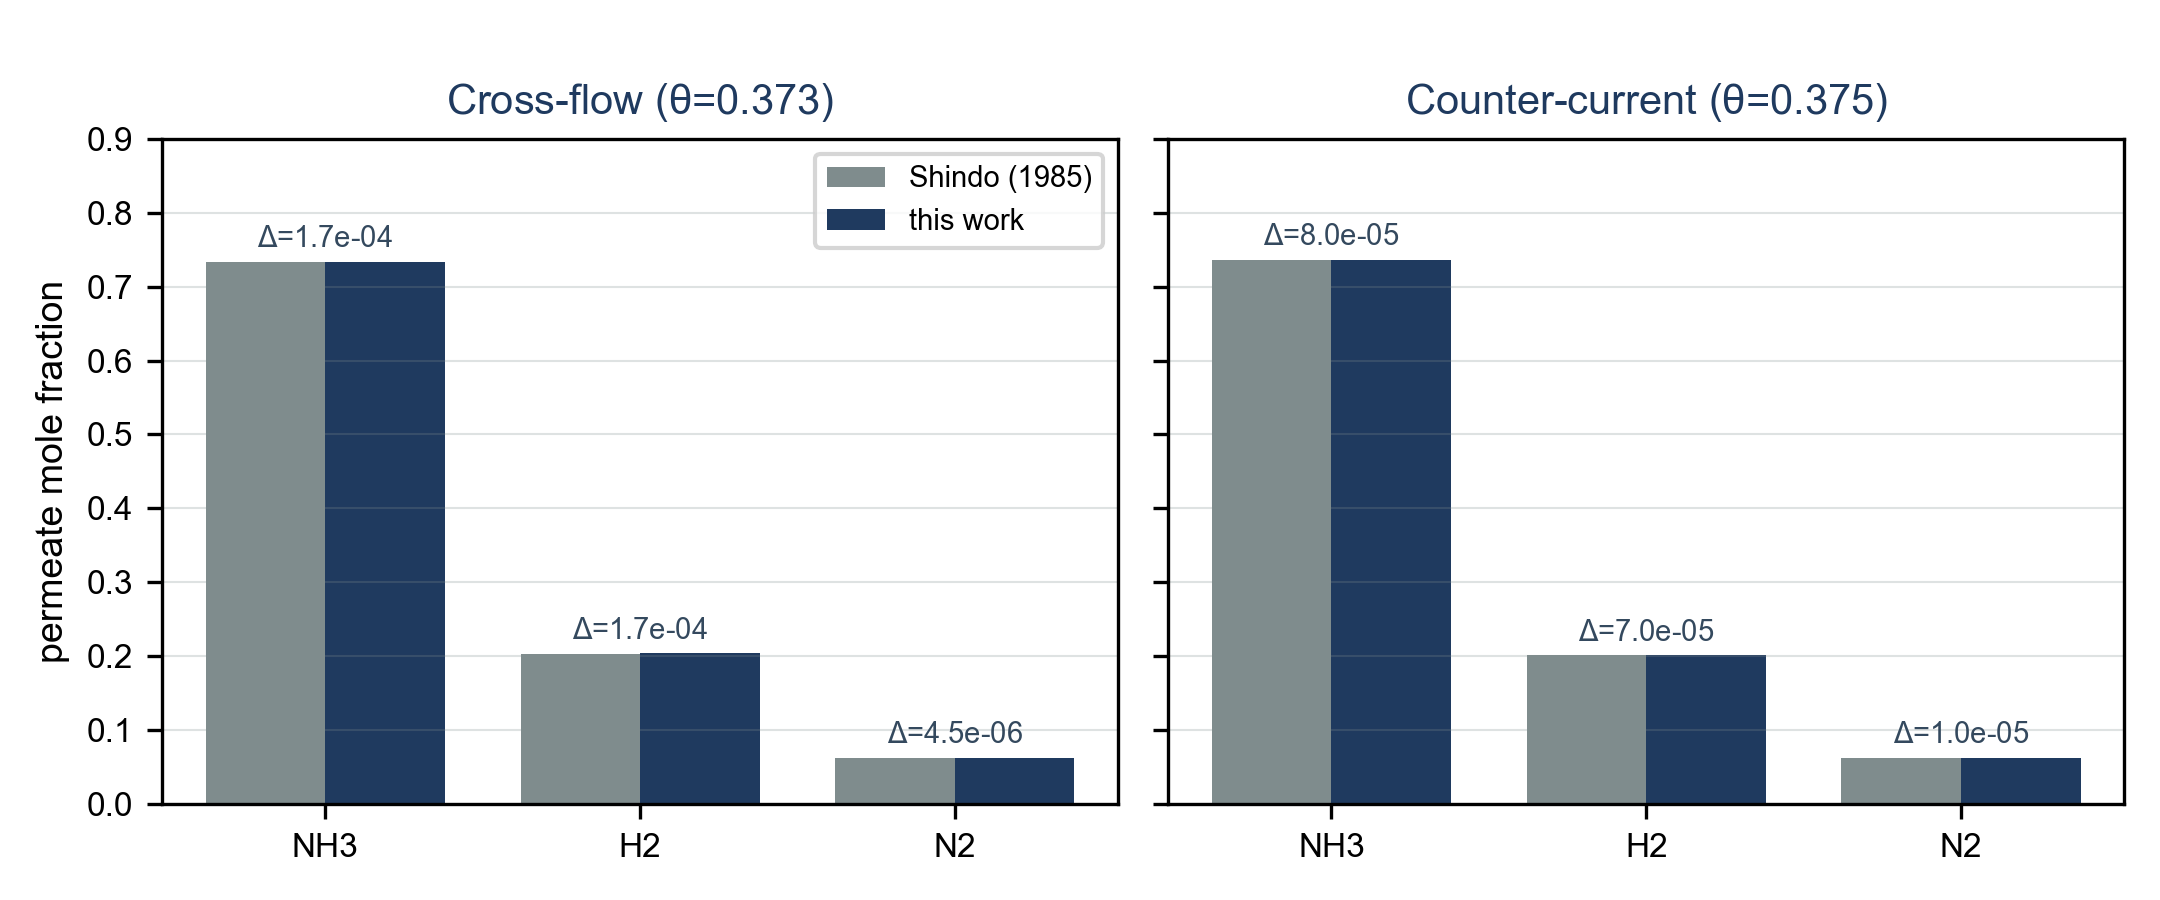
\includegraphics[width=\linewidth]{val_shindo_case1}
  \caption{Cross-flow and counter-current permeate composition for Shindo
  Case~1, this implementation against the reference values, with per-component
  absolute deviations.}\label{fig:shindo}
\end{figure*}

\subsection{Binary analytic benchmark: Weller--Steiner cross-flow}\label{sec:val-geankoplis}
Example 13.6-1 of \citet{geankoplis} solves an oxygen and nitrogen air
separation with the analytic Weller--Steiner cross-flow model
\citep{weller1950} at a feed oxygen fraction of $0.209$, an ideal selectivity of
$10$, a pressure ratio of $0.10$ and a stage cut of $0.20$. This is an
independent analytic benchmark with a fully tabulated path. The outlet
comparison is given in Table~\ref{tbl:geankoplis}, and the complete tabulated
path is matched, not only the endpoints (Fig.~\ref{fig:geankoplis}). For the
same inputs the complete-mixing model gives a poorer permeate oxygen fraction of
$0.5067$ (Example 13.4-2 of \citealt{geankoplis}), which confirms that the unit
reproduces the cross-flow physics rather than a mixed-tank idealisation.

\begin{table}[t]
\caption{Geankoplis Example 13.6-1, outlet comparison
(O\textsubscript{2}/N\textsubscript{2} cross-flow).}\label{tbl:geankoplis}
\begin{tabular*}{\tblwidth}{@{}LLL@{}}
\toprule
Quantity & \citet{geankoplis} & This work \\
\midrule
Mixed permeate $y_{\mathrm{O_2}}$ & 0.5690 & 0.5689 \\
Leading-edge local $y_{\mathrm{O_2}}$ & 0.6550 & 0.6548 \\
Retentate $x_{\mathrm{O_2}}$ at $\theta=0.20$ & 0.1190 & 0.1190 \\
\bottomrule
\end{tabular*}
\end{table}

\begin{figure}[t]
  \centering
  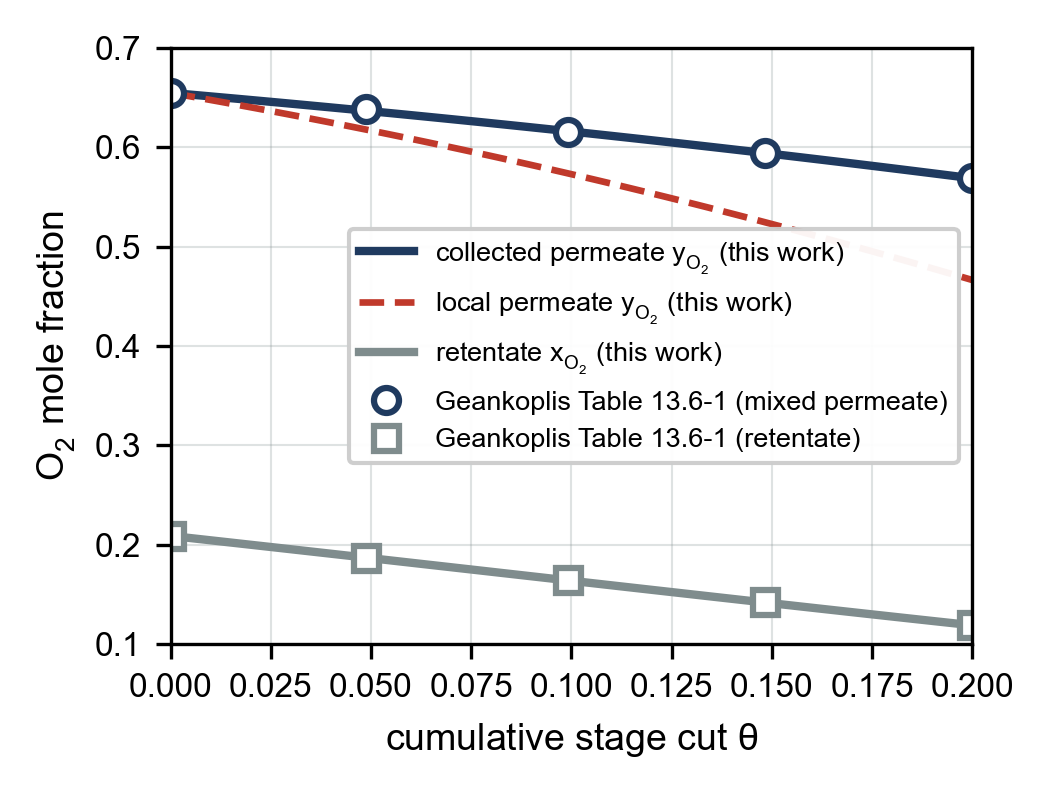
\includegraphics[width=0.85\linewidth]{val_geankoplis}
  \caption{Cross-flow oxygen and nitrogen profiles from this implementation
  (lines) against the tabulated path of \citet{geankoplis} (markers). The
  collected permeate threads every tabulated point; the local permeate is richer
  at the feed end and leaner downstream.}\label{fig:geankoplis}
\end{figure}

\subsection{Spiral-wound case set: Dias et al.}\label{sec:val-dias}
\citet{diaspinto2020} tabulate four cases spanning distinct membrane materials
and separations. Cases 1 and 2 carry the Shindo benchmark outputs reproduced
above. Cases 3 and 4 report no tabulated composition profiles. Case 3 uses
permeances given as a confidential communication in the source and is therefore
not reproduced here. Case 4 is a post-combustion carbon dioxide capture from flue
gas with the Polaris membrane, for which the source states an overall carbon
dioxide recovery of about 90\,\% rather than a composition profile. With the
permeances quoted in the source (carbon dioxide, oxygen and nitrogen of
$3.89\times10^{-7}$, $3.11\times10^{-8}$ and
$1.44\times10^{-8}$~$\mathrm{mol\,m^{-2}\,s^{-1}\,Pa^{-1}}$), a feed of 20\,\%
carbon dioxide and a pressure ratio of $0.12$, the unit reaches that 90\,\%
recovery at a stage cut of $0.36$ (permeate about 50\,\% and retentate about
3\,\% carbon dioxide). The recovery is consistent with the $\sim$90\,\% reported
for spiral-wound membrane post-combustion capture \citep{Merkel2010,diaspinto2020},
although that industrial process also uses a permeate-side sweep that the present
unit does not model.

\subsection{Hollow-fibre counter-current against experiment}\label{sec:val-aziaba}
Two counter-current hollow-fibre cases compiled by \citet{aziaba2022} exercise
the multicomponent counter-current model, an experiment by \citet{sada1992} and a
model by \citet{chowdhury2005}. Both report the cumulative permeate composition
against stage cut, which depends only on the feed, the permeance ratios and the
pressure ratio, so the membrane area is not required. For the Sada carbon
dioxide, oxygen and nitrogen separation through cellulose triacetate at feed
pressures from 5.9 to 15.7 bar, this unit's counter-current carbon dioxide curves
track the digitised reference curves closely; the residuals are a few thousandths
of a mole fraction, which is within the uncertainty of digitising the source
figure (Fig.~\ref{fig:aziaba}). For the Chowdhury
hydrogen, nitrogen, methane and argon separation at a feed pressure of 69.6 bar,
the unit reproduces the hydrogen permeate fraction stated in the source, about
$0.975$ at a stage cut of $0.30$, and preserves the correct ordering of the minor
components, provided the argon permeance is read as $7.0$ rather than the
$70$ (in units of $10^{-10}\,\mathrm{mol\,m^{-2}\,s^{-1}\,Pa^{-1}}$) listed in the
compiled table of \citet{aziaba2022}; the larger value would make argon the most
permeable of the minor components, inconsistent with the reported ordering, so it
appears to be a factor-of-ten transcription error in that compilation.

\begin{figure*}[t]
  \centering
  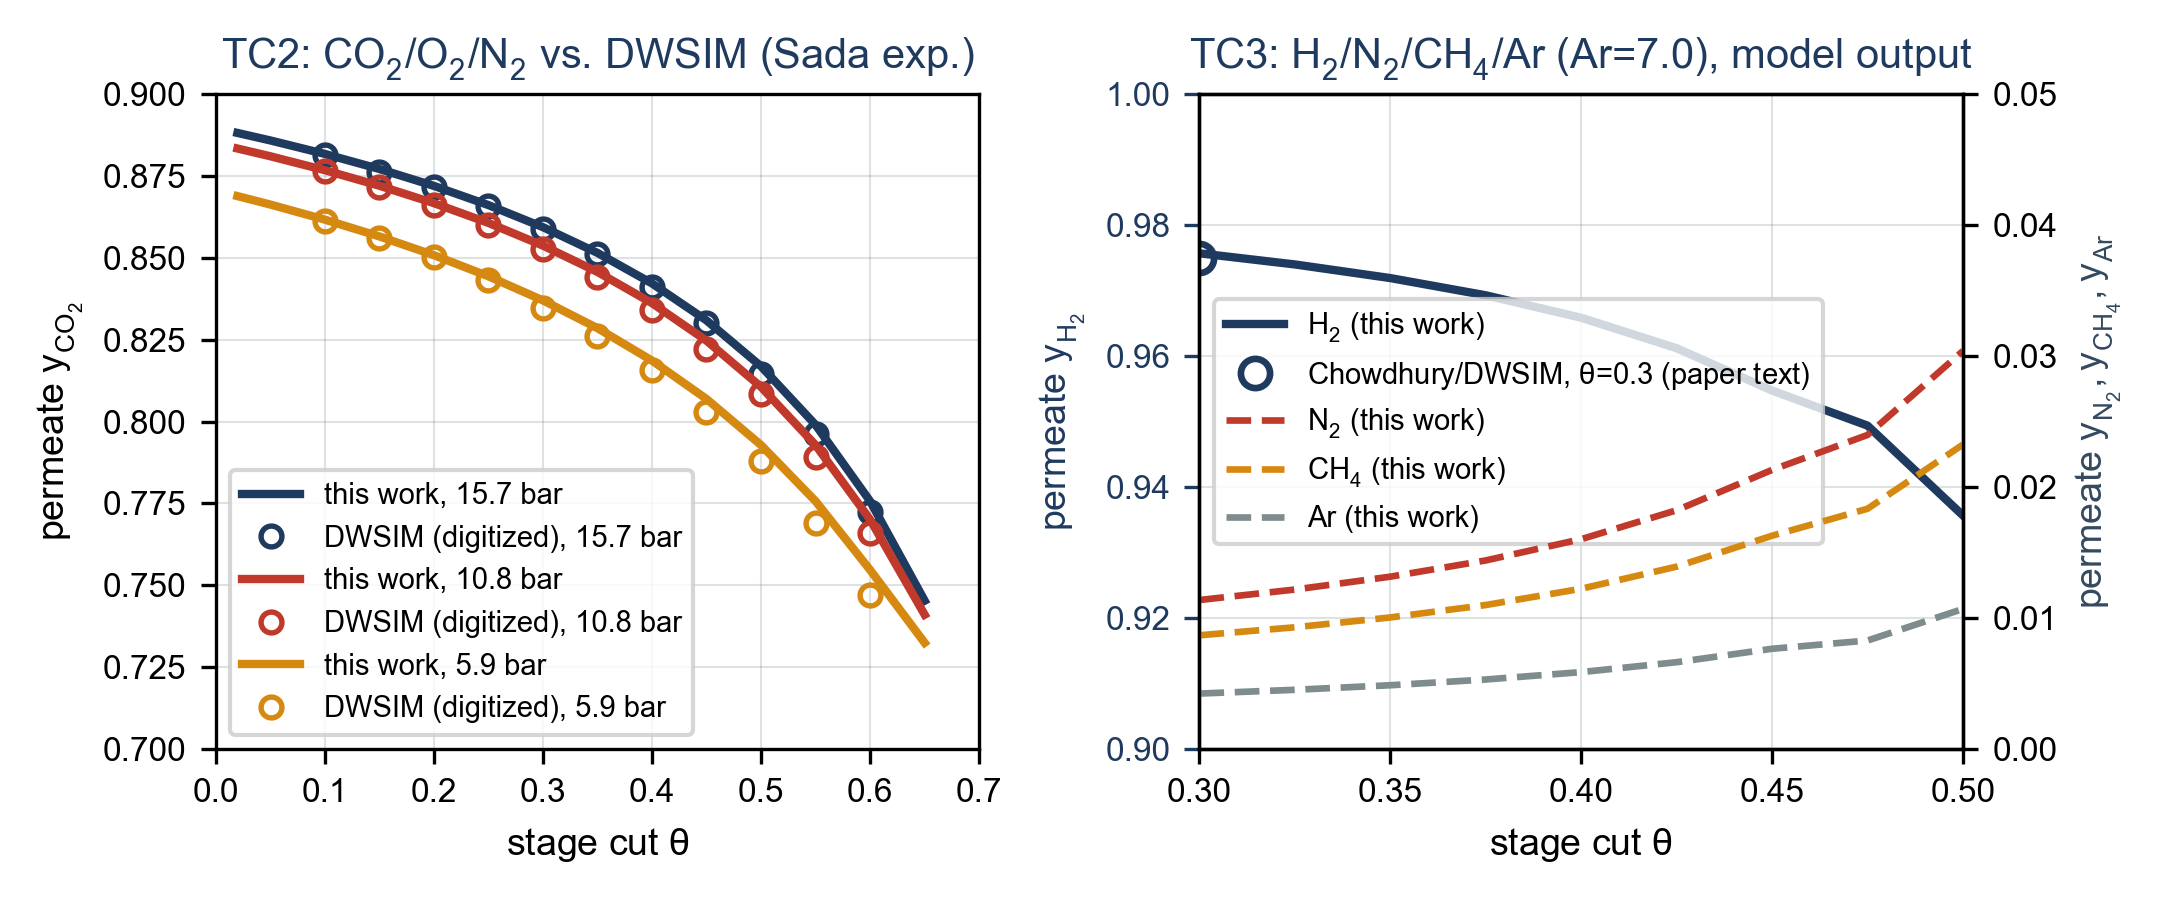
\includegraphics[width=\linewidth]{val_aziaba}
  \caption{Counter-current hollow-fibre validation. Left: carbon dioxide
  permeate against stage cut for the Sada experiment at three feed pressures,
  this solver (lines) against the digitised reference curves (circles). Right:
  the Chowdhury case with the value stated numerically in the source
  (circle).}\label{fig:aziaba}
\end{figure*}

\subsection{Air separation against measurement}\label{sec:val-airsep}
The strongest test is against measured data. \citet{dejaco2020} report twelve
operating points of a spiral-wound nitrogen and oxygen air-separation module,
with a feed of about 21\,\% oxygen, feed pressures of 205 and 274 kPa and a
permeate at 1.01 bar, spanning stage cuts from 0.04 to 0.61. Running this unit's
cross-flow solver at each point's stage cut, with the ideal selectivity of $2.54$
implied by the mid-range single-gas permeances reported in the source, reproduces
the measured permeate oxygen fraction across the whole range to a maximum
deviation of $0.010$ mole fraction (Fig.~\ref{fig:airsep}). The retentate oxygen
fraction also tracks the data except at the highest stage cuts, above about
$0.45$, where the assumption of a single permeance ratio slightly over-depletes
oxygen, consistent with real modules departing from ideal cross-flow near
exhaustion.

\begin{figure}[t]
  \centering
  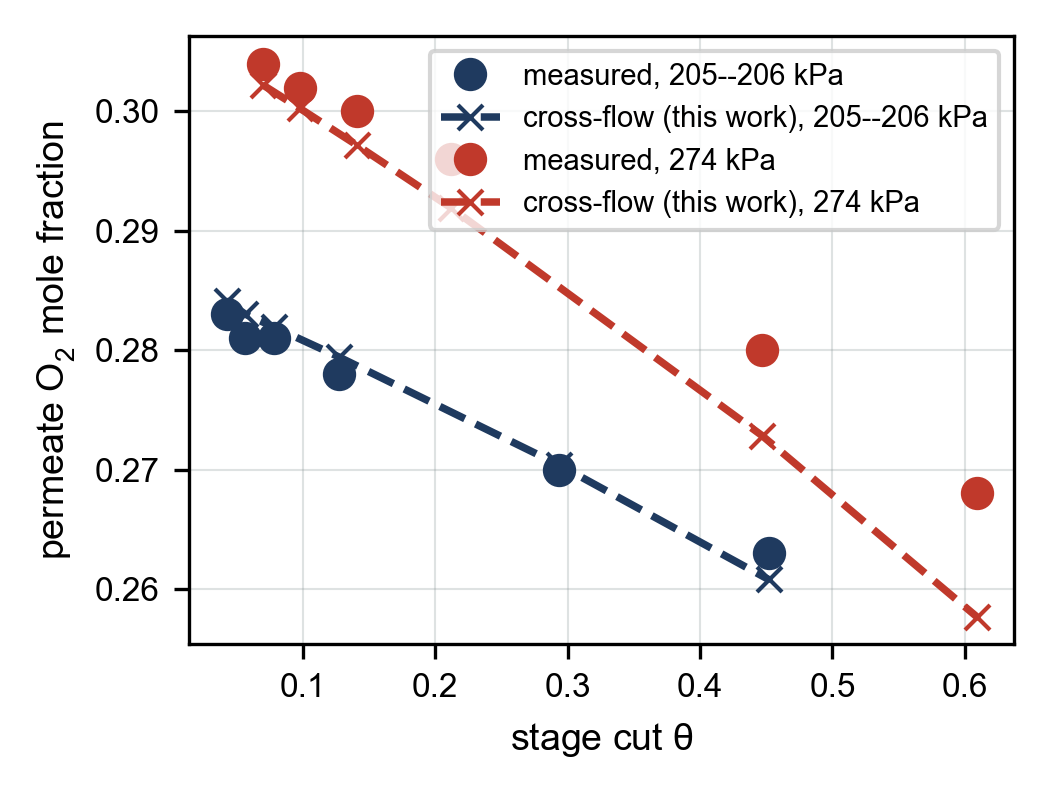
\includegraphics[width=0.85\linewidth]{val_airsep}
  \caption{Permeate oxygen fraction against stage cut for the \citet{dejaco2020}
  air-separation experiment (twelve points, two feed pressures): measured
  (filled) against this unit's cross-flow solver (dashed).}\label{fig:airsep}
\end{figure}

\subsection{Real-gas against ideal-gas driving force}\label{sec:val-igrg}
With the fugacity driving force the unit reproduces the real-gas effect directly.
For a cross-flow separation of a 10\,\% carbon dioxide, 90\,\% methane feed at
313~K, with carbon dioxide and methane permeances of $3.0\times10^{-8}$ and
$1.5\times10^{-9}$~$\mathrm{mol\,m^{-2}\,s^{-1}\,Pa^{-1}}$ (selectivity 20), a
permeate at 2 bar, and the membrane area fixed to give an ideal-gas stage cut of
$0.30$ at 40 bar, and using Peng--Robinson fugacity coefficients on the retentate
and permeate sides, the ideal-gas partial-pressure assumption progressively
over-predicts the stage cut as the feed pressure rises and the fugacity
coefficient falls below unity, by about 9\,\% at 60 bar and 15\,\% at 100 bar
relative to the real-gas value (Fig.~\ref{fig:igrg}). This is
the qualitative high-pressure trend reported by \citet{dejaco2020}. The analytic
benchmarks above are ideal-gas models and are therefore run in partial-pressure
mode to match those references, and the low-pressure air-separation experiment is
essentially unaffected because the fugacity coefficient is close to unity there.

\begin{figure}[t]
  \centering
  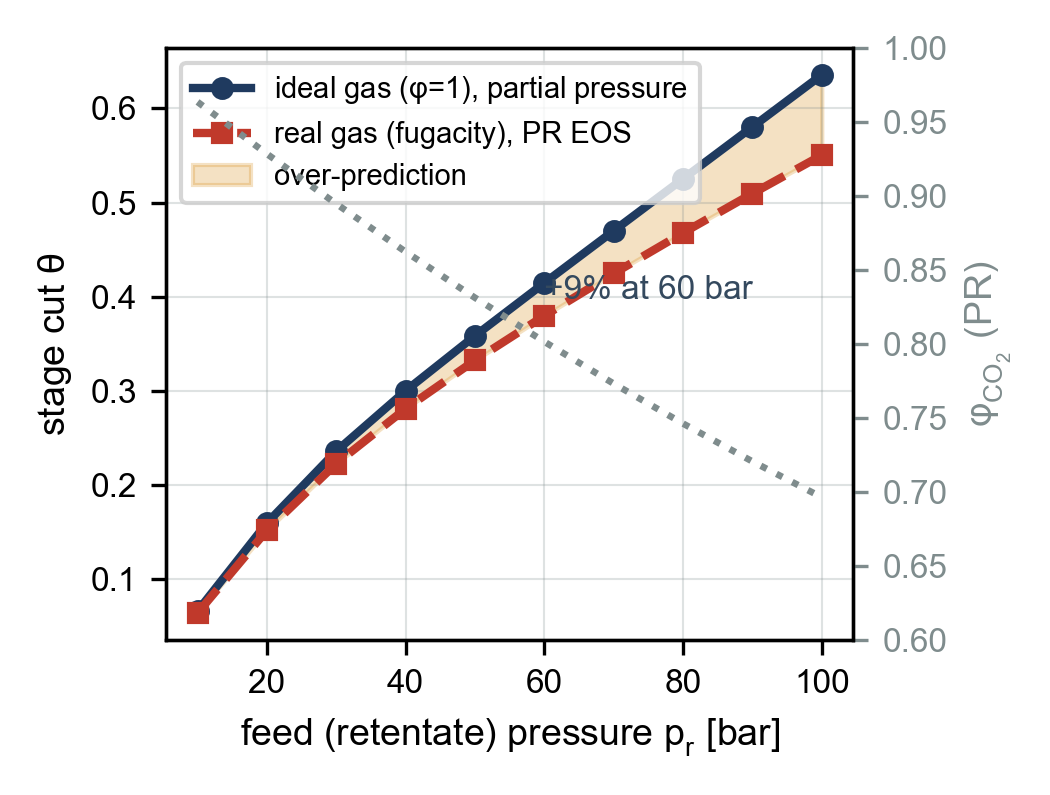
\includegraphics[width=0.85\linewidth]{val_ig_rg}
  \caption{Ideal-gas against real-gas (fugacity) stage cut versus feed pressure,
  this implementation, for a carbon dioxide and methane cross-flow at fixed area.
  The band is the ideal-gas over-prediction; the dotted line is the carbon
  dioxide fugacity coefficient from the Peng--Robinson equation of
  state.}\label{fig:igrg}
\end{figure}

A quantitative cross-check is available on the propane and propylene system that
\citet{dejaco2020} study with an equation-of-state-coupled model. Care is needed
with the convention: the difference between the ideal-gas and real-gas stage cut
can be quoted either as an absolute difference in stage-cut points or as a
relative fraction of the smaller real-gas value. The relative figure equals the
absolute one divided by the real-gas stage cut, so for this case, where the
real-gas stage cut is close to one half, the relative value is about twice the
absolute one. Reported in the absolute convention of the source, the
equation-of-state-coupled model shows an ideal-gas over-prediction of about 13
stage-cut points near 0.8 MPa. Running this unit at the same stage cut and
pressure, so that only the equation of state differs, gives the same
rise-and-fall trend at about 6 points (Fig.~\ref{fig:c3igrg}). Updating the
fugacity coefficients along the module rather than holding them at feed
conditions changes this by less than 0.02 points for propane and propylene,
because the two components have nearly identical fugacity coefficients and the
mixture value hardly changes along the module. The remaining difference is not
the constant-coefficient approximation but the fact that this unit applies the
fugacity coefficient to the driving force only, whereas the reference model
couples the equation of state through the density and velocity balances and
resolves a channel pressure drop. The driving-force correction nonetheless
captures the correct sign and trend and removes roughly half of the ideal-gas
error (about 6 of the 13 stage-cut points), a useful screening-level improvement.

\begin{figure}[t]
  \centering
  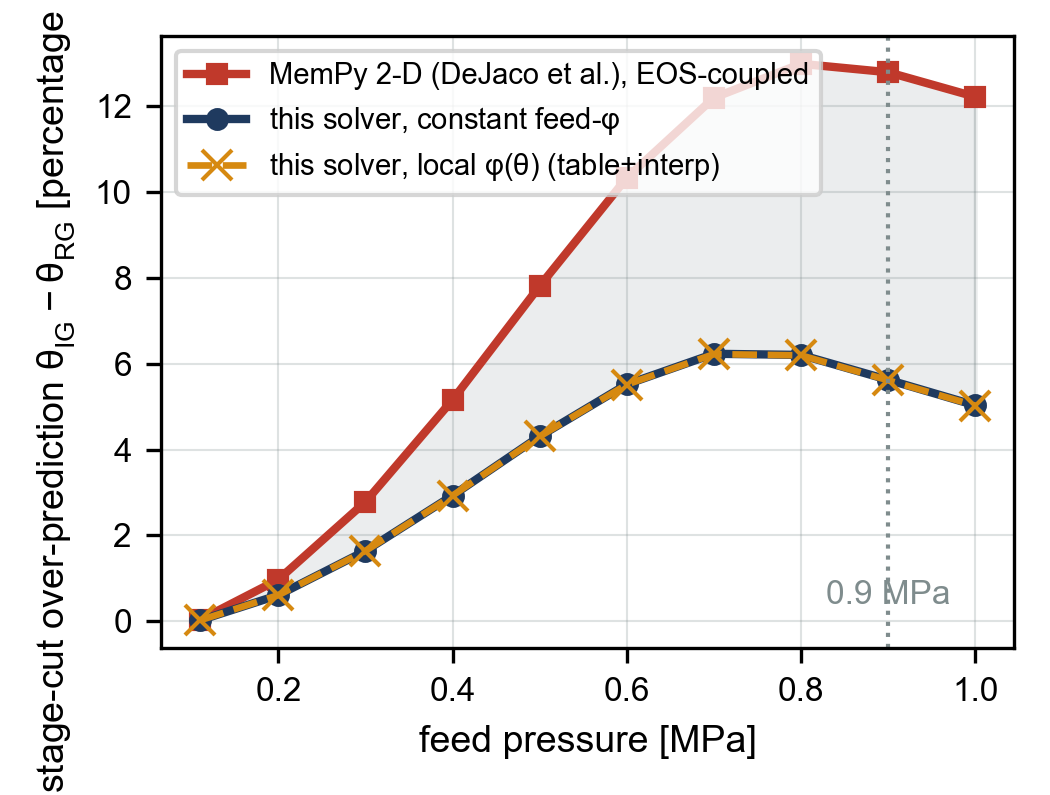
\includegraphics[width=0.82\linewidth]{val_c3_ig_rg}
  \caption{Ideal-gas stage-cut over-prediction (absolute, in stage-cut points)
  versus feed pressure for the propane and propylene system at matched stage cut:
  the equation-of-state-coupled reference model, this solver with feed-evaluated
  fugacity coefficients, and this solver with coefficients updated along the
  module.}\label{fig:c3igrg}
\end{figure}

\subsection{Energy balance: analytic limits}\label{sec:val-energy}
The adiabatic energy balance is checked against its two closed-form limits with
synthetic enthalpy providers, for a carbon dioxide and methane separation at a
stage cut of $0.30$. An ideal gas returns both outlets exactly to the feed
temperature, the correct no-Joule--Thomson limit. A fluid with a uniform
Joule--Thomson coefficient cools the permeate by exactly the coefficient times
the pressure drop while the retentate stays at the feed temperature; at a feed
pressure of 60 bar the permeate cools by 5.80 K, and energy is conserved to
better than $10^{-9}$ in relative terms (Fig.~\ref{fig:energy}).

\begin{figure}[t]
  \centering
  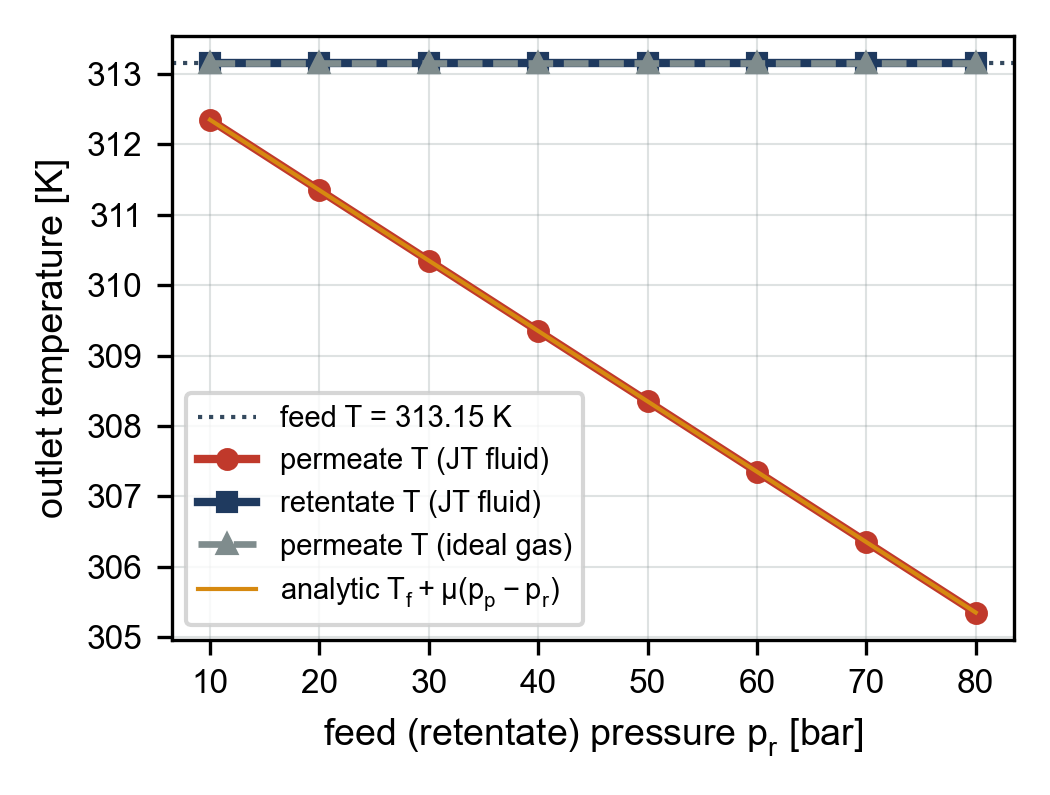
\includegraphics[width=0.8\linewidth]{val_energy_jt}
  \caption{Adiabatic energy layer: permeate and retentate outlet temperatures
  against feed pressure for a synthetic Joule--Thomson fluid, with the ideal-gas
  result and the analytic line. For this synthetic fluid, which has no excess
  enthalpy of mixing, the permeate carries all the temperature change and the
  retentate none.}\label{fig:energy}
\end{figure}

%% ============================================================================
\section{Illustrative case study}\label{sec:casestudy}
The purpose of the unit operation is that a membrane can be solved inside a
flowsheet, together with the compressors, coolers and recycle streams that
surround it and under the same property package as the rest of the flowsheet.
This section demonstrates that use on a two-stage carbon dioxide / methane
separation representative of natural gas sweetening. The configuration, a two
stage arrangement with interstage recompression and recycle of the second-stage
retentate, is the one identified by \citet{ahmad2012} as the economic optimum
for this separation. In that study the membrane was added to Aspen HYSYS as a
user-defined unit operation, which is tied to a licensed simulator and was not
released; the same configuration is built here from the released unit and the
native units of the free COCO/COFE environment.

\subsection{Flowsheet and specification}\label{sec:case-flowsheet}
The feed is a binary mixture of 10 mol\% carbon dioxide and 90 mol\% methane at
313.15~K and 60~bar, with a molar flow of 138~mol\,s$^{-1}$ (about
10~MMSCFD). The sweet-gas specification is a retentate carbon dioxide content of
2~mol\%, a representative pipeline limit and the same specification used by
\citet{ahmad2012}. The membrane has a carbon dioxide permeance of 100~GPU and a
methane permeance of 5~GPU, a carbon dioxide / methane selectivity of 20 typical
of a carbon dioxide selective polymeric membrane; a permeance of 1~GPU
corresponds to $3.348\times10^{-10}$~mol\,m$^{-2}$\,s$^{-1}$\,Pa$^{-1}$.

The flowsheet is shown as a simplified schematic in Fig.~\ref{fig:case-bfd} and
as built in COCO/COFE in Fig.~\ref{fig:case-cofe}. The fresh feed is combined
with the recycle stream and enters the primary membrane, whose area is set by a
flowsheet controller (the controller block in Fig.~\ref{fig:case-cofe}) that
adjusts the stage cut until the retentate reaches the 2~mol\% specification. The
retentate leaves as sweet gas at feed pressure. The carbon dioxide enriched
permeate leaves at 2~bar and is recompressed to 60~bar in three intercooled
stages of equal pressure ratio, $(60/2)^{1/3}\approx3.1$, set by a calculator
block (Fig.~\ref{fig:case-cofe}), and fed to the secondary membrane. The secondary permeate, at 1.2~bar, is the carbon
dioxide vent; the secondary retentate is recycled to the primary feed at a fixed
stage cut of 0.5. The flowsheet is solved in COCO/COFE with the ChemSep
Peng--Robinson property package. The compressors, intercoolers and mixer are the
environment's native units, and the two membranes obtain their enthalpies and
fugacities from the same property package through the Material Object. The
real-gas fugacity driving force and the adiabatic energy balance are both active,
so the membrane is solved consistently with the equation of state used for the
recompression train. The flowsheet file is provided in the repository.

\begin{figure*}[t]
  \centering
  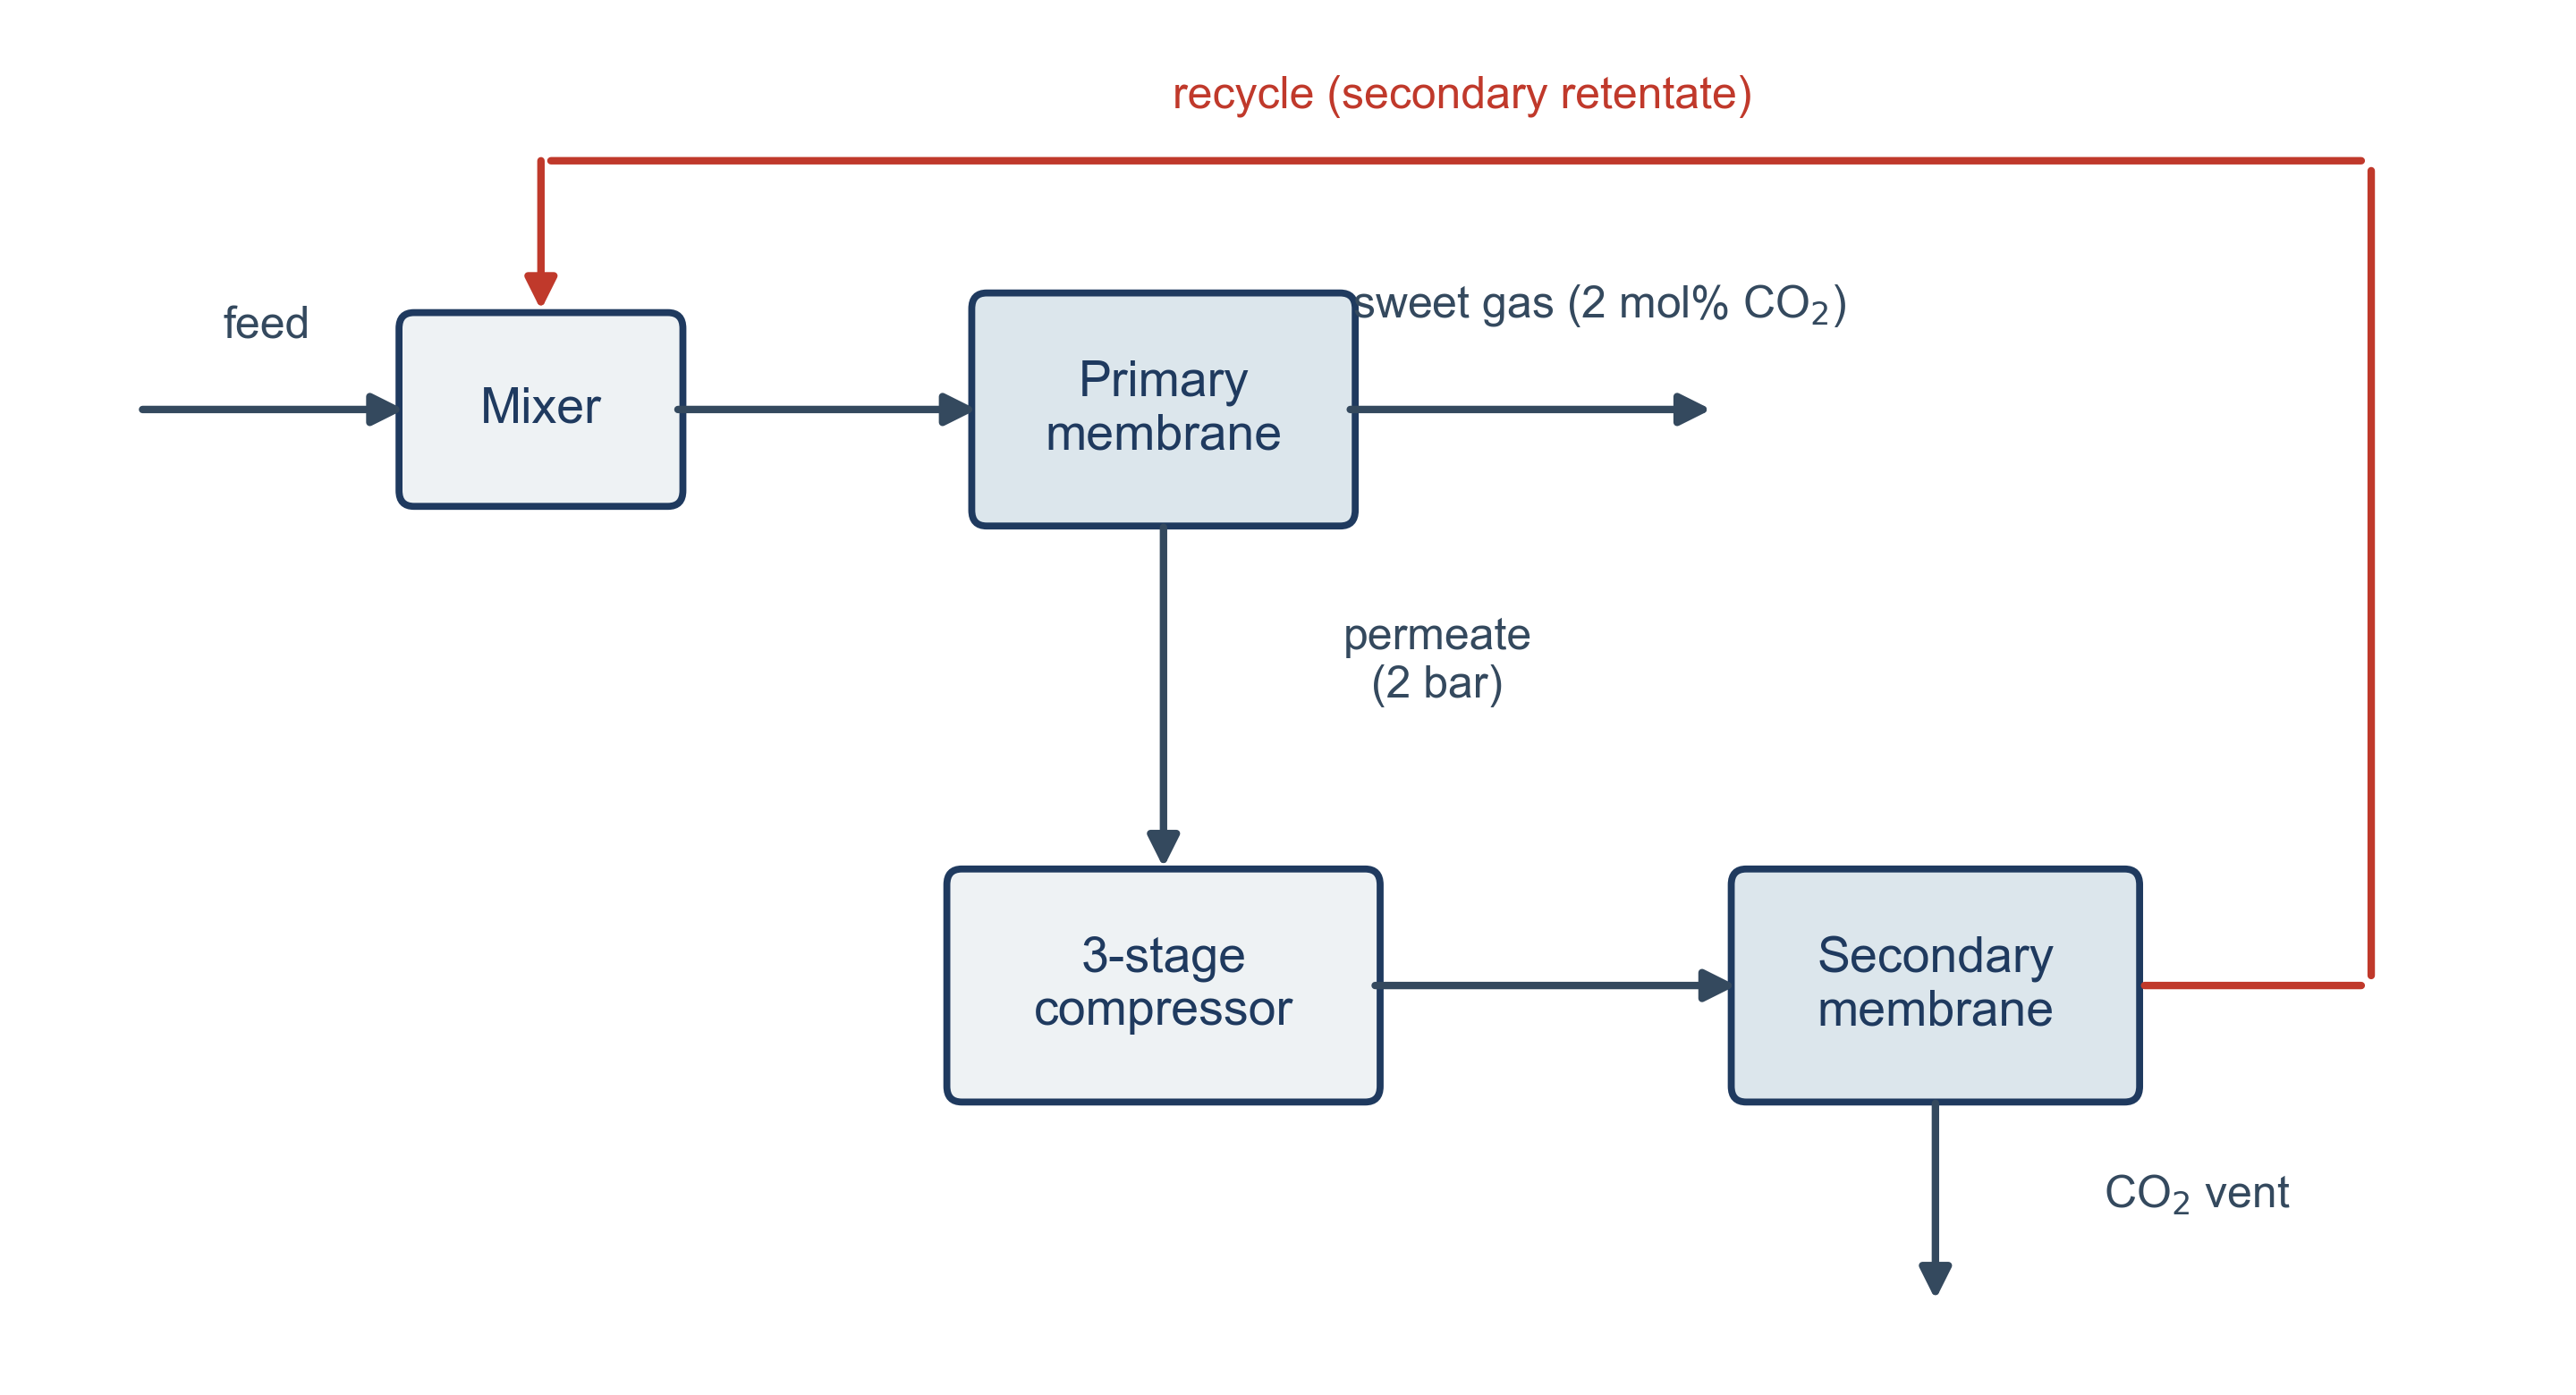
\includegraphics[width=0.86\linewidth]{case_bfd}
  \caption{Simplified schematic of the two-stage carbon dioxide / methane
  separation with interstage recompression and recycle of the second-stage
  retentate. The membranes are the unit operation described here; the mixer,
  compressor and intercoolers are the native COCO/COFE units. All streams are
  solved under one Peng--Robinson property package.}\label{fig:case-bfd}
\end{figure*}

\begin{figure*}[t]
  \centering
  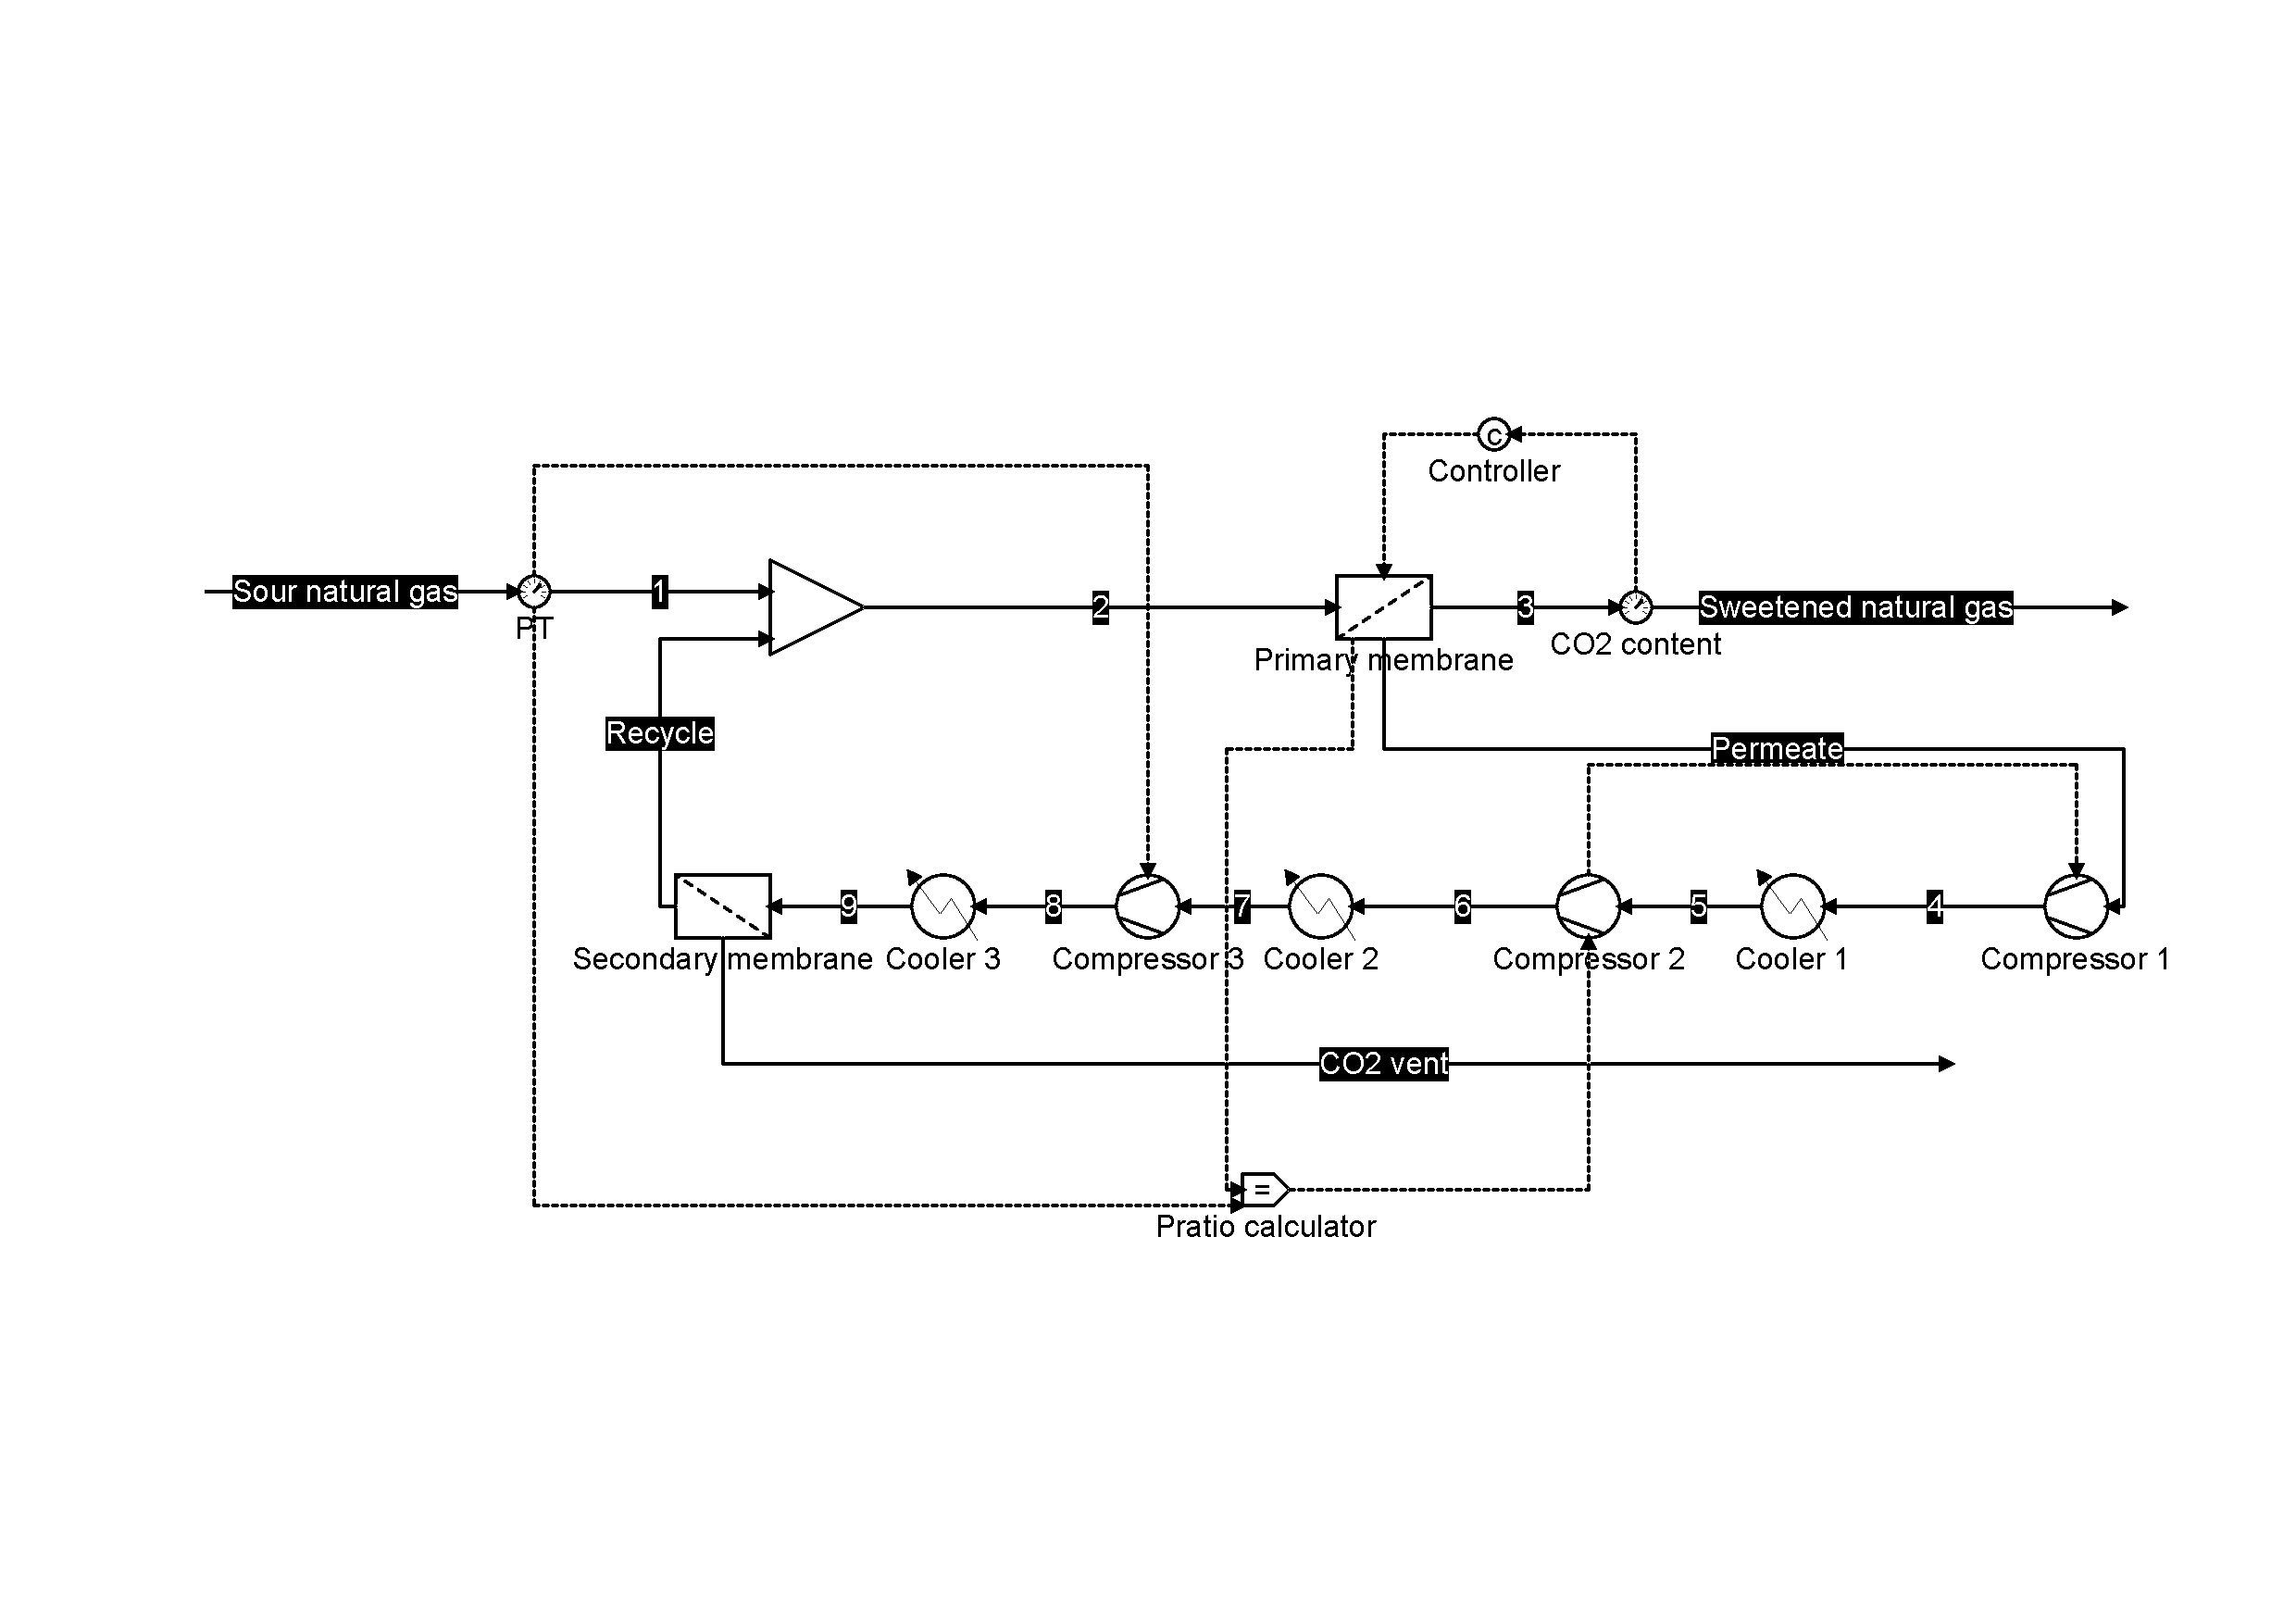
\includegraphics[width=\linewidth]{case_flowsheet}
  \caption{The same flowsheet as built in COCO/COFE. The recompression is
  resolved into three native compressor and intercooler pairs; a pressure and
  temperature indicator (PT) reads the feed, a controller adjusts the primary
  membrane area until the sweet-gas carbon dioxide content reaches the 2~mol\%
  specification, and a calculator block sets the three interstage pressures to a
  common ratio. Streams are numbered 1 to 9.}\label{fig:case-cofe}
\end{figure*}

\subsection{Base case}\label{sec:case-base}
The converged base-case results are summarised in Table~\ref{tbl:casebase}. The
sweet gas meets the 2~mol\% specification at a primary stage cut of 0.20, with a
methane recovery of 96.9\% and a carbon dioxide content in the vent of
74.4~mol\%. The primary membrane accounts for most of the total area, and the
recompression of the primary permeate requires 0.38~MW.

The parametric studies below each vary one quantity at a time and are run as COFE
parametric studies, so their membrane areas, methane recovery and recompression
power come directly from the flowsheet solved under the property package, with the
controller re-converging on the 2~mol\% specification at every point. The
feed-pressure study is run in both driving-force modes; the permeate-pressure and
selectivity studies use the real-gas fugacity driving force. A
simulator-independent reproduction of the same physics core agrees with these
solves to within about one percent on membrane area and 0.1~points on methane
recovery, and shows that an ideal-gas isentropic estimate of the recompression
power would over-predict the real-gas value by about seven percent.

\begin{table}[t]
\caption{Converged base-case results for the separation of
Fig.~\ref{fig:case-bfd}, solved in COCO/COFE with the ChemSep Peng--Robinson
property package. The values are the 2~bar point of the permeate-pressure
parametric study (Fig.~\ref{fig:case-perm}).}\label{tbl:casebase}
\begin{tabular*}{\tblwidth}{@{}LR@{}}
\toprule
Quantity & Value \\
\midrule
Sweet-gas carbon dioxide content & 2.0~mol\% \\
Methane recovery & 96.9\% \\
Carbon dioxide in vent & 74.4~mol\% \\
Primary membrane stage cut & 0.20 \\
Primary membrane area & $2.23\times10^{3}$~m$^2$ \\
Secondary membrane area & $5.1\times10^{2}$~m$^2$ \\
Total membrane area & $2.74\times10^{3}$~m$^2$ \\
Interstage compression power & 0.38~MW \\
\bottomrule
\end{tabular*}
\end{table}

\subsection{Parametric behaviour}\label{sec:case-param}
Fig.~\ref{fig:case-igrg} shows the effect of feed pressure on the required
primary membrane area between 30 and 80~bar, run as a COFE parametric study in
both driving-force modes so that the two curves differ only by the setting of the
membrane driving force. The area falls as the pressure rises, because the
transmembrane driving force increases. At every pressure the
real-gas fugacity driving force returns a larger required area than the ideal
partial-pressure model, and the difference widens with pressure, from about 15\%
at 30~bar to about 24\% at the 60~bar base case and about 29\% at 80~bar. This is
the same real-gas deviation quantified in Section~\ref{sec:val-igrg}; at
sweetening pressures a partial-pressure model under-sizes the membrane by a
margin that is not negligible for design.

\begin{figure}[t]
  \centering
  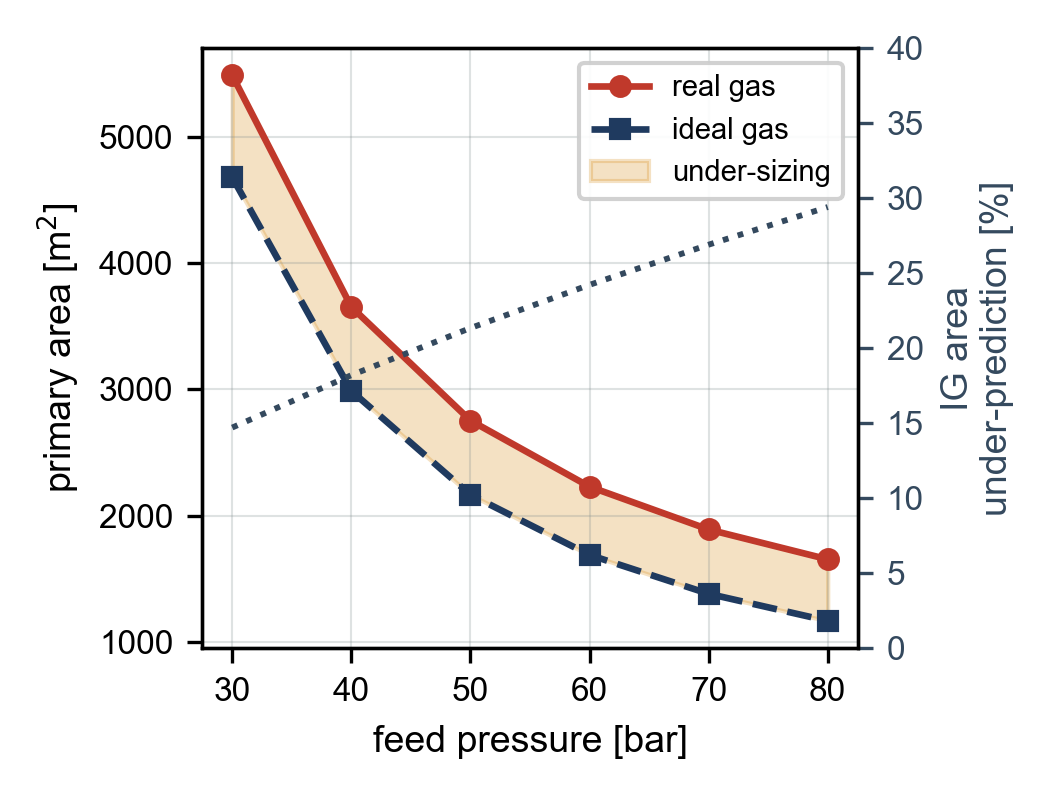
\includegraphics[width=\linewidth]{case_realgas}
  \caption{Required primary membrane area against feed pressure for the base-case
  specification, from a COFE parametric study run with the real-gas fugacity
  driving force and with the ideal partial-pressure driving force. The right axis
  shows the fraction by which the partial-pressure model under-predicts the
  area.}\label{fig:case-igrg}
\end{figure}

Fig.~\ref{fig:case-perm} shows the effect of the primary permeate pressure
between 1.5 and 6~bar. Throughout the study the secondary stage cut and the vent
pressure are held fixed and only the primary stage cut floats, set by the
controller, which holds the sweet-gas specification at every point. A lower
permeate pressure raises the driving force, so the total membrane area falls, from
about $5.8\times10^{3}$~m$^2$ at 6~bar to about $2.5\times10^{3}$~m$^2$ at
1.5~bar, and the methane recovery rises from 90.7 to 97.4\%. The recompression
power is highest at the lowest permeate pressure, about 0.40~MW at 1.5~bar, and
passes through a shallow minimum of about 0.365~MW near 4~bar, because a lower
permeate pressure raises the compression ratio but also reduces the permeate flow
that has to be recompressed. The base case at 2~bar lies below the pressure of
minimum power; relative to that optimum it gives a smaller area and a higher
methane recovery at the cost of a small increase in recompression power, about
0.38 against 0.365~MW.

\begin{figure}[t]
  \centering
  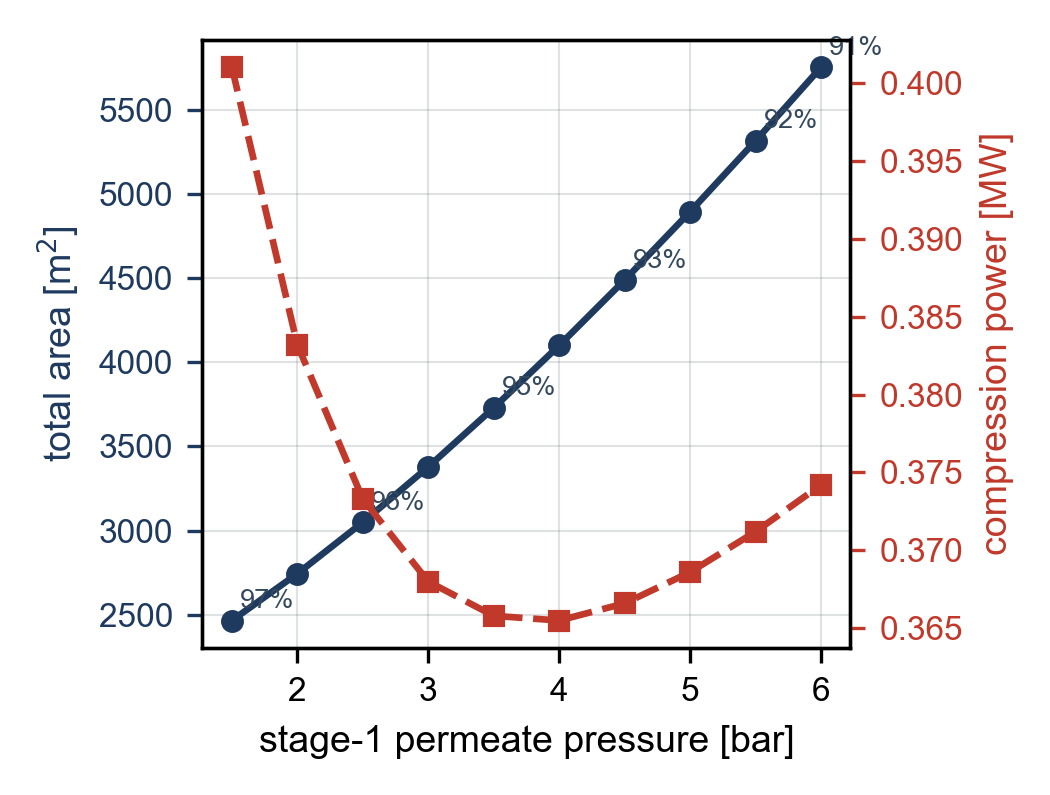
\includegraphics[width=\linewidth]{case_permeate}
  \caption{Total membrane area and recompression power against the primary
  permeate pressure from a COFE parametric study, with the methane recovery
  labelled at each point. Lower permeate pressure reduces the area and improves
  the recovery; the recompression power has a shallow minimum near
  4~bar.}\label{fig:case-perm}
\end{figure}

Fig.~\ref{fig:case-alpha} shows the effect of the carbon dioxide / methane
selectivity between 5 and 40 at a fixed carbon dioxide permeance, obtained by
varying the methane permeance of both membranes in a COFE parametric study. The
methane recovery rises steeply at low selectivity and saturates at high
selectivity, from about 78\% at a selectivity of 5 to about 99\% at a selectivity
of 40. The selectivity of 5 corresponds to the cellulose-acetate membrane used by
\citet{alqaheem2021}, who reports carbon dioxide and methane permeances of 67 and
13~GPU; the low recovery at that selectivity is consistent with the low
hydrocarbon recovery reported there for a high carbon dioxide feed. The total area
is comparatively insensitive to selectivity, between about $2.7\times10^{3}$ and
$3.0\times10^{3}$~m$^2$, but the recompression power rises sharply at low
selectivity, from about 0.30~MW at a selectivity of 40 to about 1.0~MW at a
selectivity of 5, because more methane permeates and must be recompressed and
recycled.

\begin{figure}[t]
  \centering
  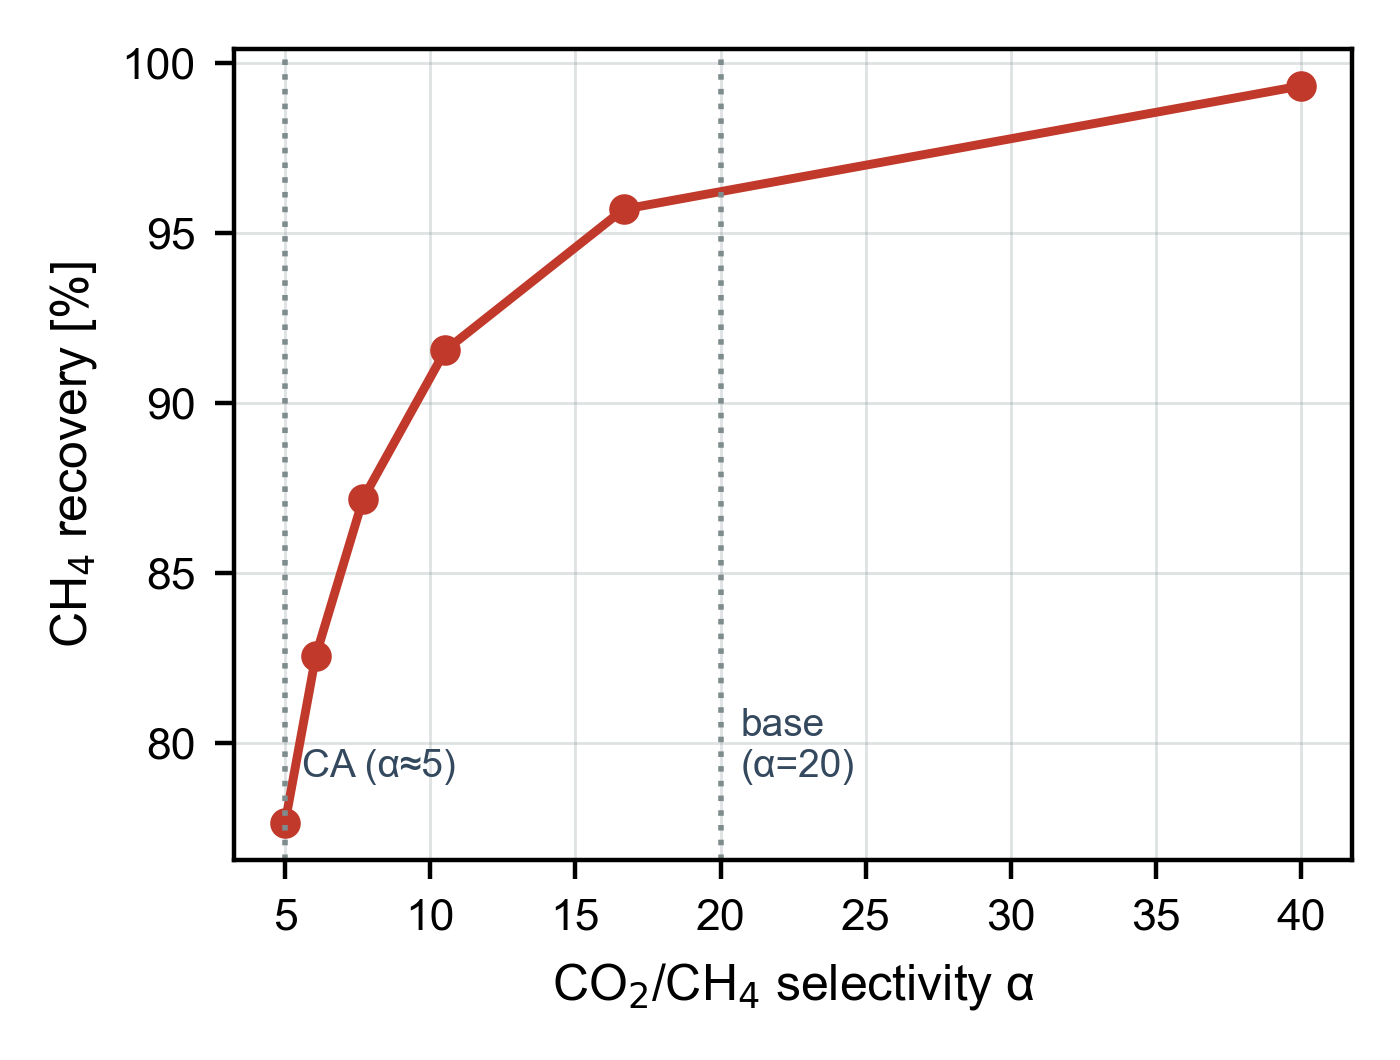
\includegraphics[width=\linewidth]{case_selectivity}
  \caption{Methane recovery against the carbon dioxide / methane selectivity at a
  fixed carbon dioxide permeance, from a COFE parametric study varying the methane
  permeance of both membranes. The selectivity of the cellulose-acetate membrane
  of \citet{alqaheem2021} and the base-case selectivity are
  marked.}\label{fig:case-alpha}
\end{figure}

The case study demonstrates the intended use of the unit. The membrane is solved
together with the recompression train, the intercoolers and the recycle under a
single property package in a free environment, with the real-gas and
non-isothermal options active, and the parametric trends reproduce established
behaviour for this separation without leaving the flowsheet or re-implementing
the model.

%% ============================================================================
\section{Discussion}\label{sec:discussion}
Because the unit obtains its thermodynamics from the flowsheet property package
and complies with the CAPE-OPEN standard, a membrane can be studied together with
the compressors, heat exchangers and recycle streams that surround it, under the
same equation of state as the rest of the flowsheet, and in more than one
compliant environment. This addresses the practical limitations of the earlier
routes reviewed in Section~\ref{sec:intro}. Custom units built inside a commercial
simulator \citep{ahmad2012,bocciardo2013,salano2025} are tied to a licensed tool
and are generally not released; a membrane reconstructed from a component splitter
and a spreadsheet is laborious and specific to one flowsheet
\citep{alqaheem2024accuracy}; a model kept in an external numerical environment
and connected through a plug-in requires that environment to be installed
\citep{alqaheem2024coco}; and rigorous open codes run outside the simulators and
need a dedicated toolchain \citep{dejaco2020,aziaba2022,bozorg2019}. The unit
presented here is instead distributed as a compiled component that registers in
the free COCO/COFE environment, and in any other compliant environment, without a
separate numerical environment, an external solver, or recompilation, with the
source released under an open licence.

The model has clear limitations, some shared with the models it is compared
against. The real-gas correction is applied to the driving force only and not to
the density and velocity balances or to a channel pressure drop, so it captures
the sign and trend of the high-pressure deviation and removes a useful fraction
of the ideal-gas error, but it does not reproduce a fully coupled
equation-of-state model (Section~\ref{sec:val-igrg}). The retentate channel
pressure drop is neglected, and the permeances are taken constant, independent of
temperature, pressure and composition, which is adequate for screening but not
for membranes with strongly composition-dependent or plasticising behaviour. Flux
is capped at zero rather than allowed to reverse; this cap is inert in cross-flow,
where the local driving force is structurally non-negative
(Section~\ref{sec:model-assumptions}), but in the co- and counter-current patterns
it suppresses the physically real back-permeation that occurs where the bulk
permeate partial pressure exceeds the retentate value, a one-way-permeation
approximation. The
energy balance is a lumped adiabatic reduction that assigns outlet temperatures
rather than a distributed non-isothermal model such as that of
\citet{fontoura2022}, and the separation is treated as decoupled from
temperature. These choices keep the unit robust and portable inside a flowsheet
solver, which is the intended use, and they define the directions for further
work: coupling the equation of state through the transport balances, adding a
channel pressure drop, allowing composition- and temperature-dependent
permeances, and extending the same architecture to a wider set of unit
operations.

%% ============================================================================
\section{Conclusions}\label{sec:conclusions}
A gas-permeation membrane unit operation has been presented that is openly
available, ready to use in a free process modelling environment, and validated
against independent references. The unit implements the solution-diffusion
cross-flow, co-current and counter-current models with a choice of
partial-pressure or real-gas fugacity driving force and an optional adiabatic
energy balance, and delegates all thermodynamics to the flowsheet property
package through the CAPE-OPEN Material Object. The physics are held in a
simulator-independent core, and a thin adapter exposes the model as a CAPE-OPEN
unit operation that registers in COCO/COFE, and in any other compliant
environment, without external numerical tools or recompilation. The unit
reproduces the Shindo multicomponent benchmark and the Weller--Steiner analytic
cross-flow solution to an absolute agreement of order $10^{-4}$, reproduces the
hollow-fibre counter-current data compiled by Aziaba, tracks the permeate
composition of a twelve-point air-separation experiment to within $0.010$ mole
fraction, and recovers the $\sim$90\,\% carbon dioxide recovery reported for a
spiral-wound flue-gas capture case. The real-gas driving force captures the high-pressure deviation
from ideal-gas behaviour that a partial-pressure model misses. A two-stage carbon
dioxide / methane sweetening flowsheet, solved in the free environment with
interstage recompression and recycle, illustrates the unit in use and reproduces
both the real-gas sensitivity of the required membrane area and the optimality of
the two-stage recycle configuration reported for this separation. By combining an
open licence, a free flowsheet environment and a standard interface, the unit
makes rigorous, validated membrane calculations available for flowsheet-level
studies without the barriers of the earlier approaches, and its architecture
provides a basis for further membrane and other unit-operation models.

%% ---- Back matter ------------------------------------------------------------
\section*{Code availability}
The source code is available at [[repository URL]] under the MIT licence; the
release described here is archived at [[Zenodo DOI]]. The technical reference
(model, numerics, validation) is provided in the repository.

\printcredits

\bibliographystyle{cas-model2-names}
\bibliography{references}

\end{document}
